%%%%%%%%%%%%%%%%%%%%%%%%%%%%%%%%
%	APS RevTeX4 class 
%%%%%%%%%%%%%%%%%%%%%%%%%%%%%%%%
\documentclass[aps, prd, twocolumn, showpacs, superscriptaddress,
preprintnumbers, nofootinbib]{revtex4-1}

%%%%%%%%%%%%%%%%%%%%%%%%%%%%%%%%
%	Packages
%%%%%%%%%%%%%%%%%%%%%%%%%%%%%%%%
\usepackage{graphicx}
\usepackage{amsmath}
\usepackage[dvipsnames]{xcolor}
\usepackage{ulem}
\usepackage{enumitem}
\usepackage{hyperref}
\usepackage{braket}
\usepackage[utf8]{inputenc}


\hypersetup{ 
    pdfnewwindow=true,      % links in new window
    colorlinks=true,       % false: boxed links; true: colored links
    linkcolor=blue,          % color of internal links
    citecolor=blue,        % color of links to bibliography
    filecolor=blue,      % color of file links
    urlcolor=blue        % color of external links
}  

%%%%%%%%%%%%%%%%%%%%%%%%%%%%%%%%
%	New commands
%%%%%%%%%%%%%%%%%%%%%%%%%%%%%%%%
\newcommand{\be}{\begin{eqnarray}}
\newcommand{\ee}{\end{eqnarray}}
\newcommand{\non}{\nonumber \\}
\newcommand{\com}[1]{{\color{orange}\textbf{[COMMENT}\footnote{\color{orange}\textit{#1}}]}}

%%%%%%%%%%%%%%%%%%%%%%%%%%%%%%%%
%	Document
%%%%%%%%%%%%%%%%%%%%%%%%%%%%%%%%
\begin{document}

%%%%%%%%%%%%%%%%%%%%%%%%%%%%%%%%
%	Title
%%%%%%%%%%%%%%%%%%%%%%%%%%%%%%%%
\title{Towards the Minimal Spectrum of Excited Baryons}

%%%%%%%%%%%%%%%%%%%%%%%%%%%%%%%%
%	Author List
%%%%%%%%%%%%%%%%%%%%%%%%%%%%%%%%
\author{J. Landay}
\email{jlanday@gwmail.gwu.edu}
\affiliation{Department of Physics, The George Washington University, Washington, DC 20052, USA}

\author{K. Nakayama}
\email{nakayama@uga.edu}
\affiliation{Department of Physics and Astronomy, The University of Georgia, Athens, GA 30602, USA}

\author{M. D\"oring}
\email{doring@gwu.edu}
\affiliation{
Institute for Nuclear Studies and Department of Physics, 
The George Washington University, Washington, DC 20052, USA}
\affiliation{Theory Center, Thomas Jefferson National Accelerator Facility, Newport News, VA 23606, USA}

\author{H. Haberzettl}
\email{helmut@gwu.edu}
\affiliation{
Institute for Nuclear Studies and Department of Physics, 
The George Washington University, Washington, DC 20052, USA}

\author{M. Mai}
\email{maximmai@email.gwu.edu}
\affiliation{Department of Physics, The George Washington University, Washington, DC 20052, USA}


\preprint{JLAB-THY-17-XXXX}

%%%%%%%%%%%%%%%%%%%%%%%%%%%%%%%%
%	Abstract
%%%%%%%%%%%%%%%%%%%%%%%%%%%%%%%%
\begin{abstract}
\com{Redo}
We present an analysis of the reaction $K^-p\to K\Xi$ using the
Least Absolute Shrinkage and Selection Operator (LASSO)
in combination with criteria from information theory 
and $K$-fold cross validation. These methods are not yet widely known
in the analysis of excited hadrons but 
will become relevant in the era of precision spectroscopy.
The principle is first illustrated with synthetic data; then, its feasibility for real data is demonstrated.
\end{abstract}

\pacs{
11.80.Et, % Partial-wave analysis
02.70.Rr, % General statistical methods
25.20.-x, % Photonuclear reactions
}

\maketitle



%%%%%%%%%%%%%%%%%%%%%%%%%%%%%%%%
%	Introduction
%%%%%%%%%%%%%%%%%%%%%%%%%%%%%%%%

\section{Introduction} \label{sec:intro}

\com{Only placeholder text to be able to cite papers. Text is totally Dada. MICHAEL'S RESPONSIBILITY}

Were follow Ref.~\cite{Jackson:2015dva}. See also Ref.~\cite{Jackson:2013bba} for the possibility of a model-independent determination of quantum numbers of excited cascade states.

Previous work in Ref.~\cite{Landay:2016cjw} Can be used in the analysis of experimental data in search for exotic  mesons or to sort out the nature of ``bumps'' in the amplitude~\cite{Jackura:2017amb, Molina:2017iaa, Pilloni:2016obd}.

Similarly has been used in analysis of optical potential~\cite{Agadjanov:2016mao} or in general three-body problem, e.g., Refs.~\cite{Briceno:2016mjc,Hammer:2017kms,Hammer:2017uqm} or Ref.~\cite{Mai:2017vot,Kamano:2011ih} for general fit problems in the finite and infinite volume, respectively. For two-body scattering on the lattice, general unknown parametrization~\cite{Briceno:2016mjc,Doring:2011vk,Doring:2011ip,Doring:2011nd,Doring:2013glu} or the fit of meson-baryon data and pseudoscalar meson photoproduction~\cite{Doring:2010ap, Huang:2011as, Ronchen:2012eg, Ronchen:2014cna, Ronchen:2015vfa}.

Bonn Gatchina~\cite{Anisovich:2011fc, Collins:2017sgu}, ANL-Osaka~\cite{Kamano:2013iva, Kamano:2014zba, Kamano:2015hxa}. Last two are strgeness -1. Other strangeness -1 are: Cesar~\cite{Fernandez-Ramirez:2015tfa}. Other piN: Manley~\cite{Shrestha:2012ep}, SAID~\cite{Workman:2012jf, Workman:2012hx, Workman:2016irf, Tiator:2016btt}, Mart (KL)~\cite{Mart:2017mwj}; DMT and MAID~\cite{Kamalov:2000en, Chiang:2002vq, Tiator:2010rp, Drechsel:1998hk, Drechsel:2007if}. Giessen~\cite{Shklyar:2014kra, Cao:2013psa}.

Wunderlich paper~\cite{Wunderlich:2016imj}. Model selection MIT~\cite{Guegan:2015mea, Williams:2017gwf}, Nys and Ryckebusch~\cite{DeCruz:2012bv,DeCruz:2011xi} bayesian inference; model discrimination~\cite{Nys:2016uel}


\section{Toy Model Formalization}

We first considered (synthetic) data addresses the transition $\bar K^-p\to K\Xi$ via polarized and unpolarized differential cross sections 
(1 MeV$^2=389.4\,\text{b}$) given by
\begin{align}
\frac{d\sigma}{d\Omega}=(|g|^2+|h|^2) \frac{k_f}{k_i}
\qquad\text{ and }\qquad
\frac{d\sigma}{d\Omega}P=\frac{2 \space \text{Re}(g)h^{*}}{|g|^2+|h|^2} \, \frac{d\sigma}{d\Omega}\,,
\end{align}
respectively, for $W$ being the total energy of system, and $m$ denote the masses of the mesons and baryons.
The spin-flip and non-flip amplitudes $g_I$ and $h_I$ for the total Isospin of the reaction\footnote{$\braket{\Xi^0 K^0 | p K^-}= - \frac{1}{2}\braket{K\Xi(1,0)|\bar KN (1,0)}- \frac{1}{2}\braket{K\Xi(0,0)|\bar KN (0,0)}$ and 
{$\braket{\Xi^- K^+ | p K^-}= - \frac{1}{2}\braket{K\Xi(1,0)|\bar KN (1,0)}+ \frac{1}{2}\braket{K\Xi(0,0)|\bar KN (0,0)}$}} $I=0,1$ are related to the partial waves via

%\begin{widetext}
\begin{equation}
\begin{split}
g_I&=\sum_{J=1}^{\text{jmax}} \frac{(2J+1)}{2 \sqrt{k_f  k_i}} \biggl[d^J_{\frac{1}{2} \frac{1}{2}}(\theta)[\tau^{J(J-\frac{1}{2})}_I+\tau^{J(J+\frac{1}{2})}_I]\cos(\frac{\theta}{2}) \\
& + d^J_{\frac{-1}{2} \frac{1}{2}}(\theta)[\tau^{J(J-\frac{1}{2})}_I-\tau^{J(J+\frac{1}{2})}_I]\sin(\frac{\theta}{2})\biggr] 
\end{split}
\end{equation}
and
\begin{equation}
\begin{split}
h_I&=-i\sum_{J=1}^{\text{jmax}} \frac{(2J+1)}{2 \sqrt{k_f  k_i}} \biggl[d^J_{\frac{1}{2} \frac{1}{2}}(\theta)[\tau^{J(J-\frac{1}{2})}_I+\tau^{J(J+\frac{1}{2})}_I]\sin(\frac{\theta}{2}) \\
&- d^J_{\frac{-1}{2} \frac{1}{2}}(\theta)[\tau^{J(J-\frac{1}{2})}_I-\tau^{J(J+\frac{1}{2})}_I]\cos(\frac{\theta}{2})\biggr].
\end{split}
\end{equation}


For a given quantum numbers $(I,J,L)$, we assume the following general parametrization of the latter
\begin{equation}
\begin{gathered}
\tau(W)= \left(a\,e^{-\alpha^2 (\frac{k_f(W)}{\Lambda})^2} -x\,e^{i\Phi} \frac{\Gamma}{2(W-M+i \frac{\Gamma}{2})} \right)\\
\times \left(\frac{k_f(W)}{\Lambda} \right) ^{L+\frac{1}{2}} \left( e^{i \phi} \right)
\end{gathered}
\end{equation}
where cutoff is fixed as $\Lambda=10^3 \text{ MeV}$, and $a,\alpha, \phi,\Phi,x, \Gamma,M$ are the free (real) parameters of the toy-model. Note that 
the latter are all different for different partial waves with the last four parameters describing resonance parameters.  


To avoid that the fit can perfectly reproduce the true solution, the synthetic data were generated using a slightly different parametrization (including an additional constant term $b$) of the background in the partial wave solutions,
\begin{equation}
\begin{gathered}
\tau(W)= \biggl((a+b\frac{k_f(W)}{\Lambda}) e^{-\alpha^2 (\frac{k_f(W)}{\Lambda})^2}\\
-x\,e^{i\Phi} \frac{\Gamma}{2(W-M+i \frac{\Gamma}{2})} \biggr)\times \left(\frac{k_f(W)}{\Lambda} \right) ^{L+\frac{1}{2}} \left( e^{i \phi} \right).
\end{gathered}
\end{equation}
These solutions were used at uniformly distributed $W$, and applying a perturbation with uniform Gauss error bars to generate the data. Furthermore, 4 resonances were included, appearing in the channels $S_{0,1}$, $P_{1,1}$, $D_{0,5}$, $D_{1,5}$. The partial waves corresponding to the data generated can be seen in  Fig.~\ref{fig:Fig1}, whereas the data itself can be seen in Figs.~\ref{fig:Fig2} and ~\ref{fig:Fig3}.


\begin{figure}
\begin{center}
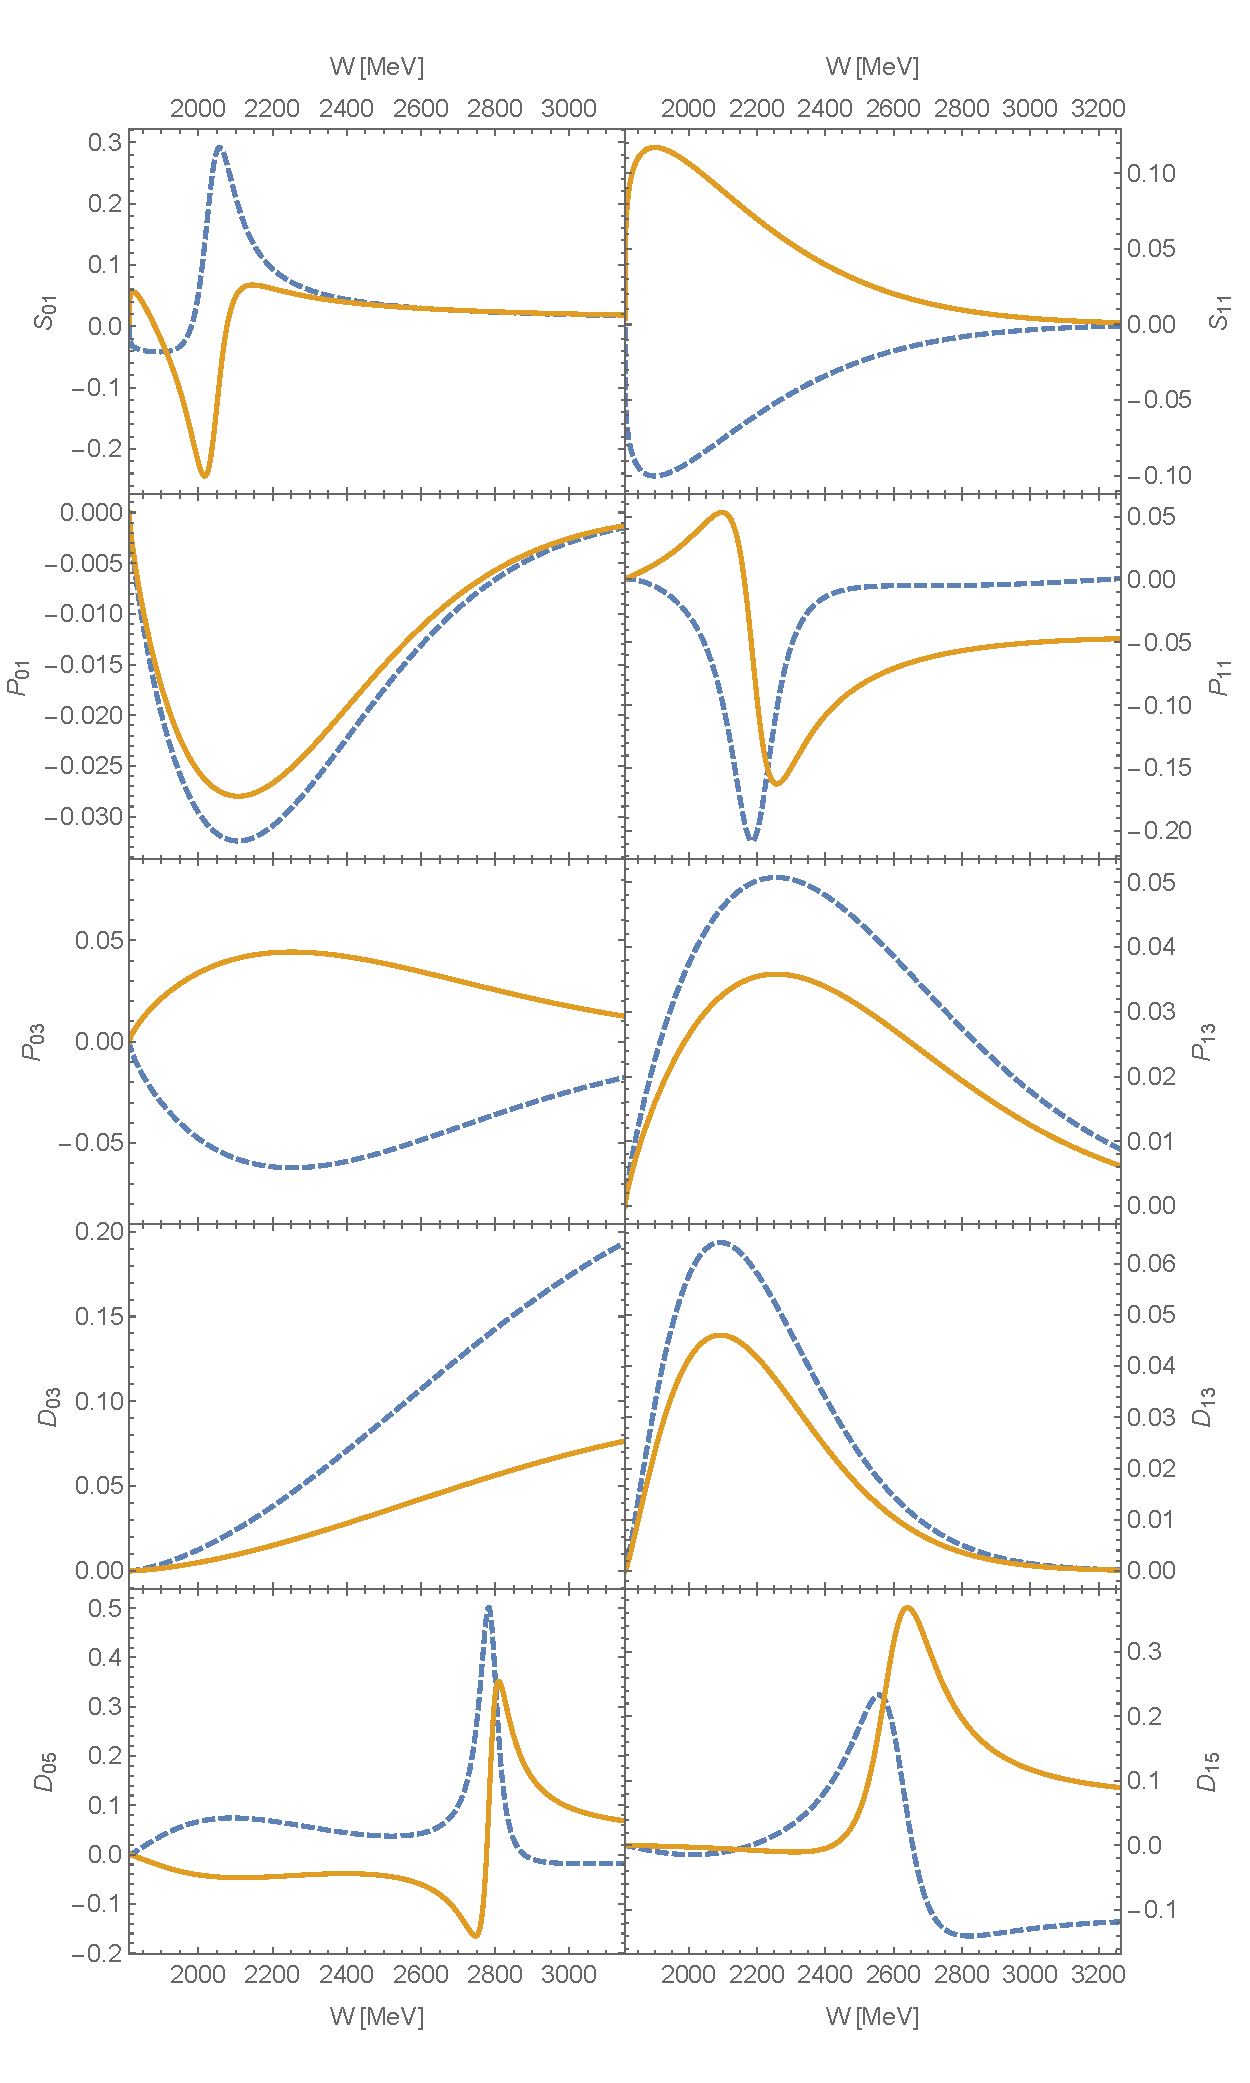
\includegraphics[width=0.99\linewidth,trim=0 1cm 0 3cm]{Fig2.pdf}
\end{center}
\caption{Partial waves of the synthetic data for the considered Isospin channels. Blue dashed and orange solid lines show the real and imaginary parts, respectively.}
\label{fig:Fig1}
\end{figure}





\begin{figure}
\begin{center}
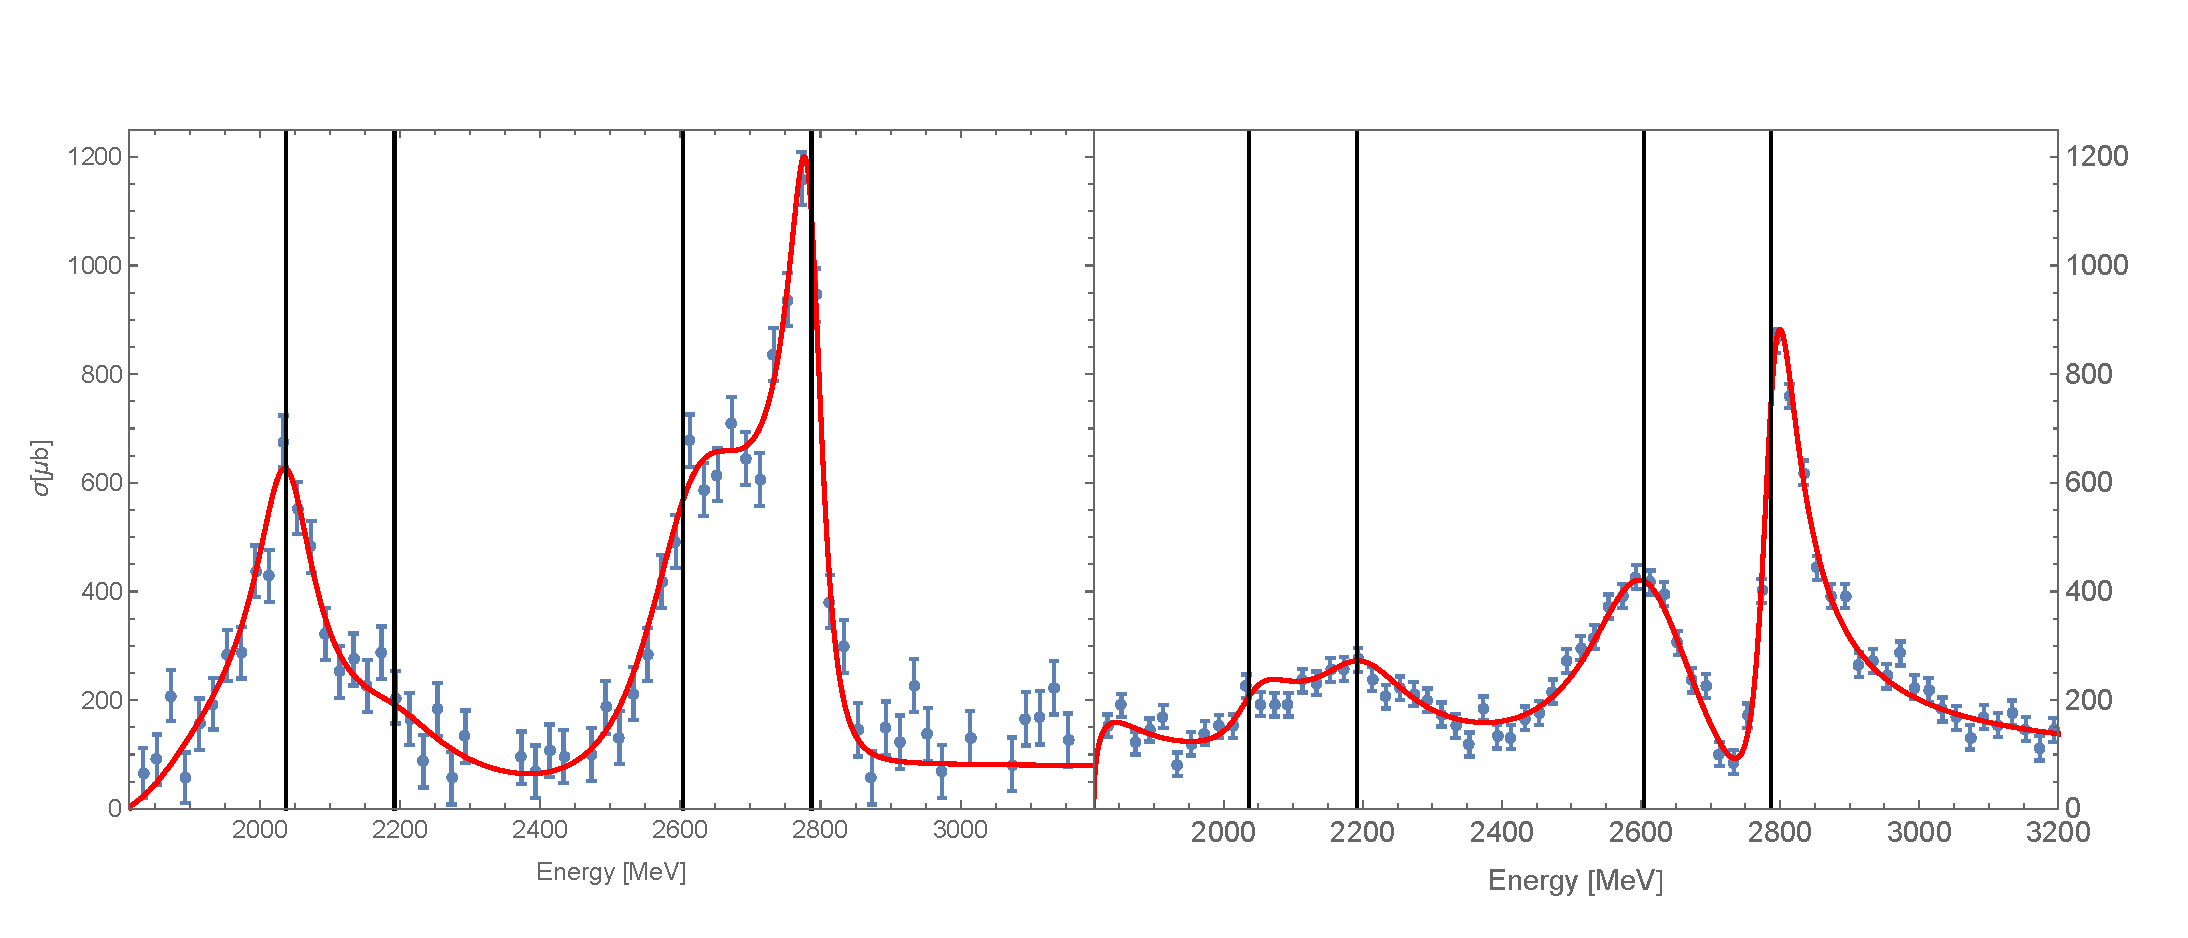
\includegraphics[width=.99\linewidth]{Fig1.pdf}
\caption{Synthetic data for the total cross sections in blue for the generating function in red. The black vertical lines correspond to the resonances masses.}
\label{fig:Fig2}
\end{center}
\end{figure}


\begin{figure}
\begin{center}
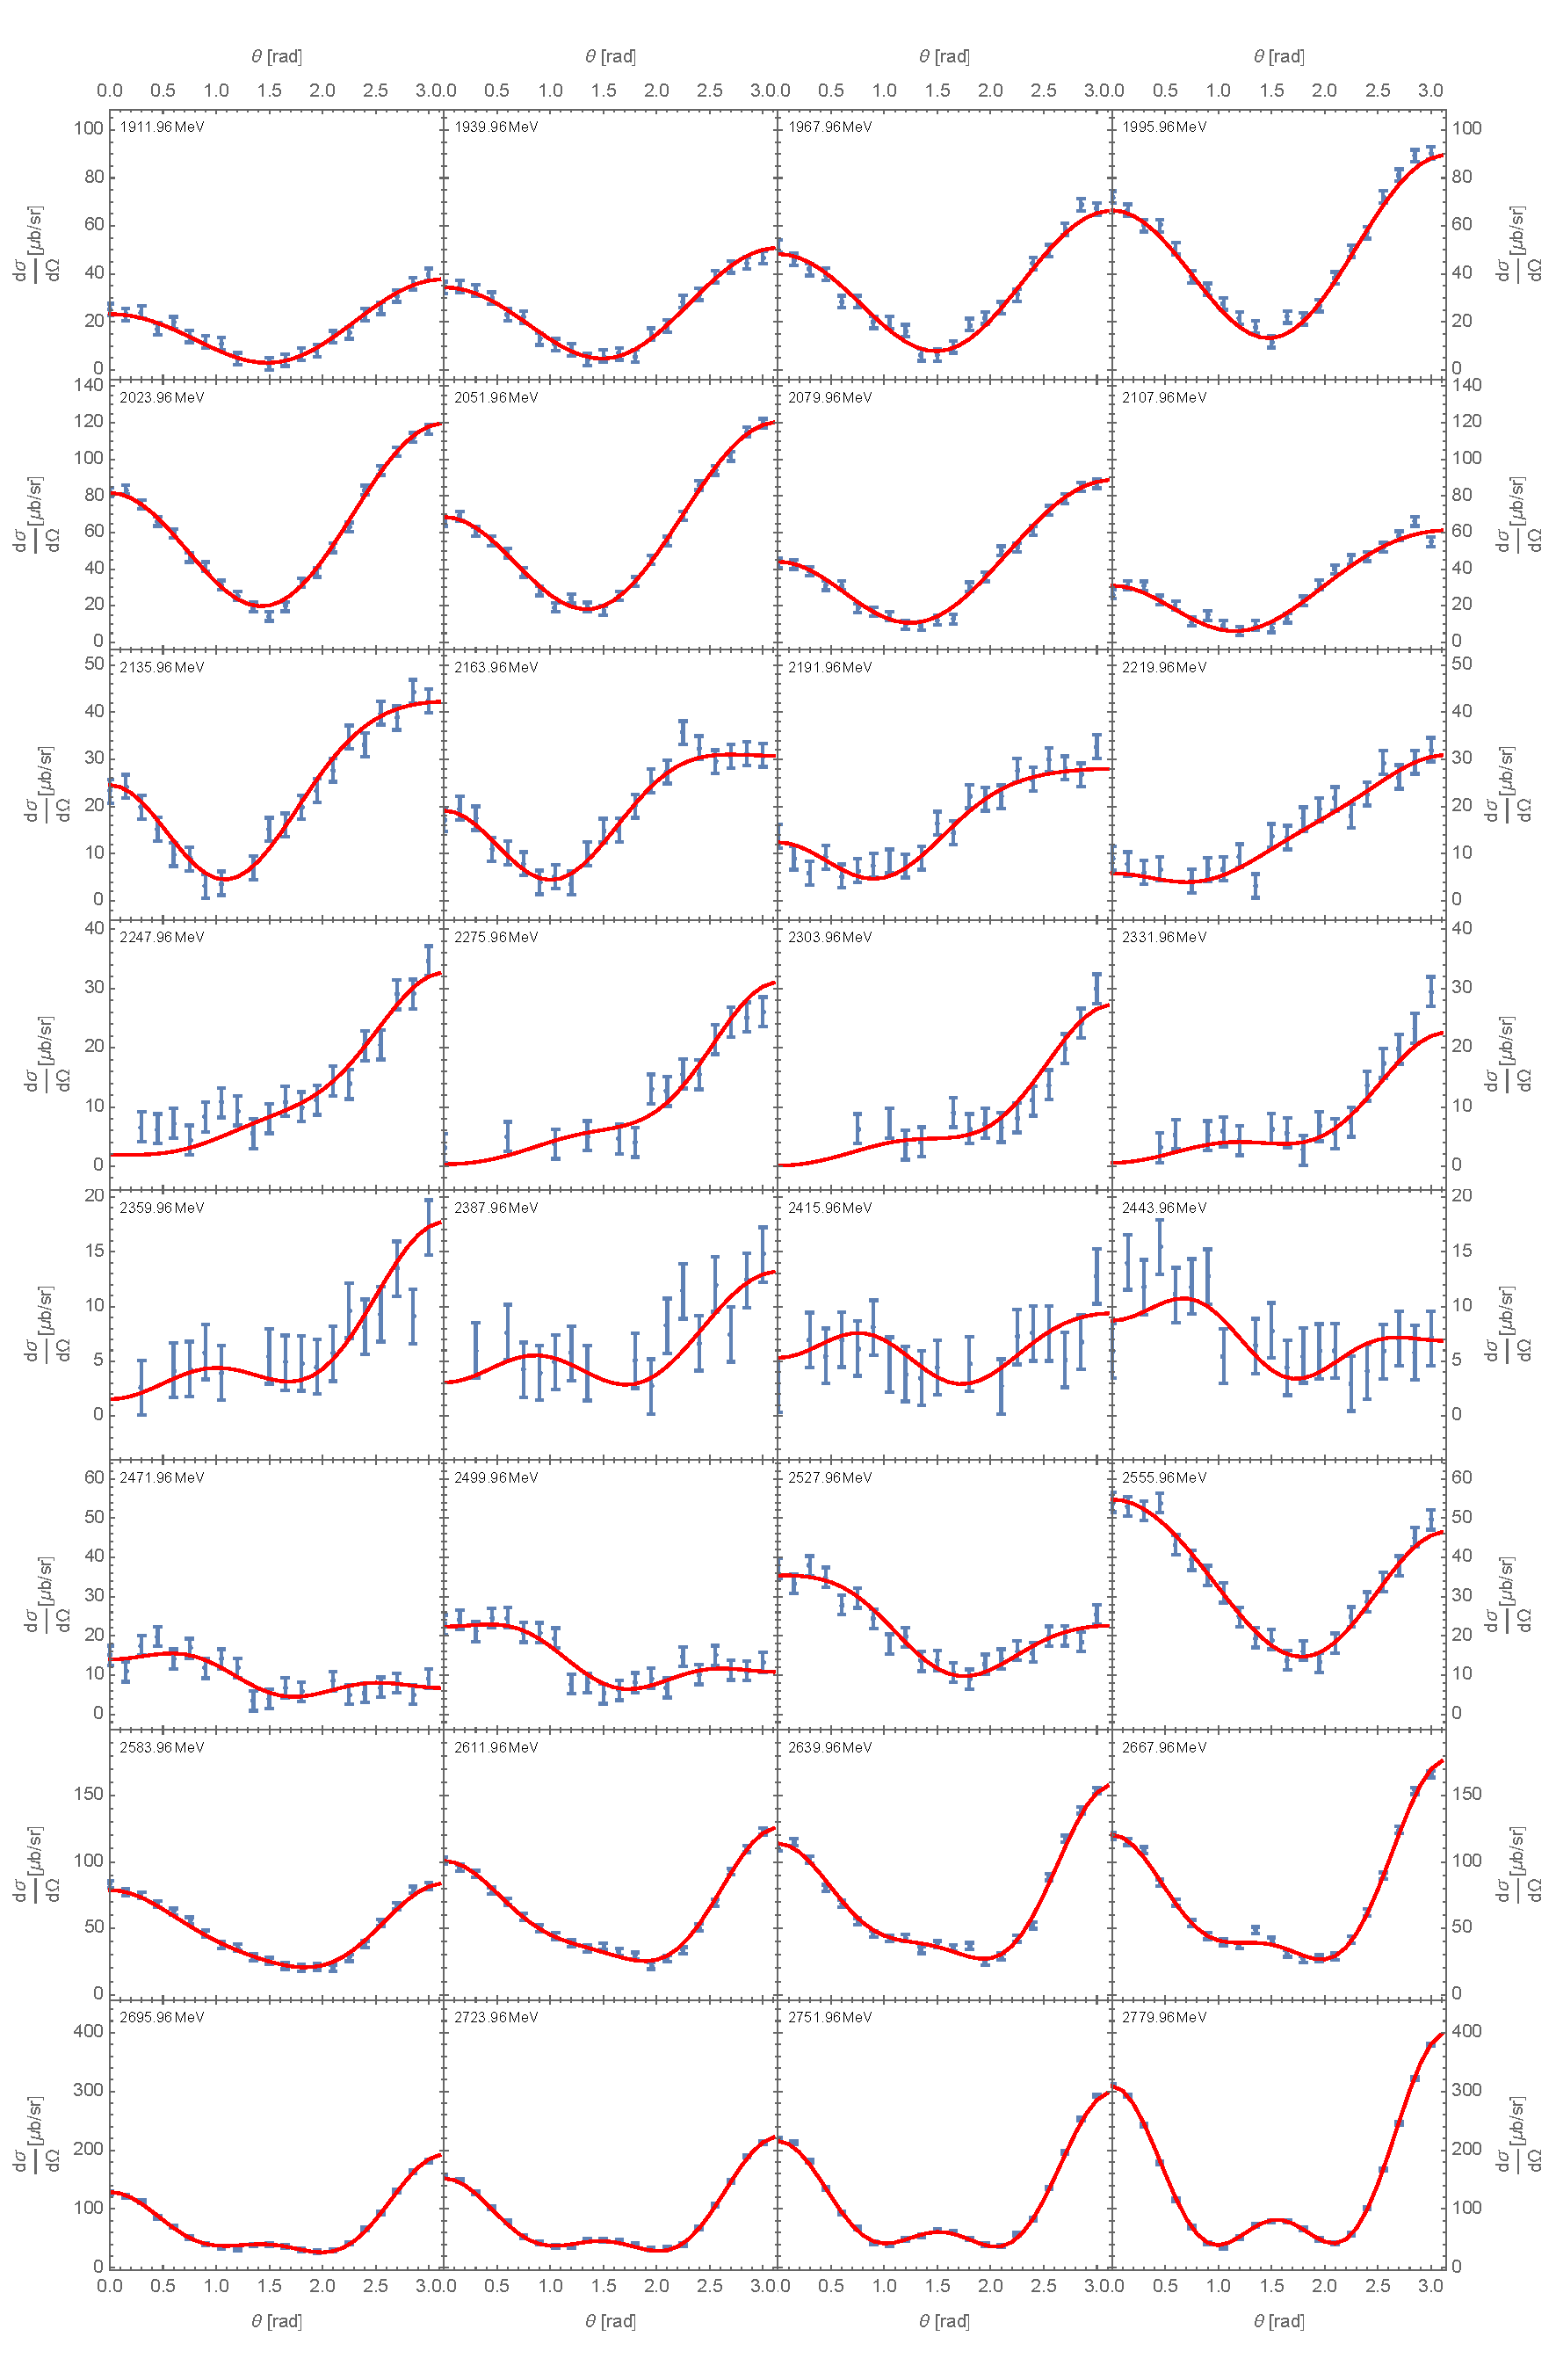
\includegraphics[width=0.49\linewidth,trim=1cm 0cm 0cm 7cm]{Diff1.pdf}
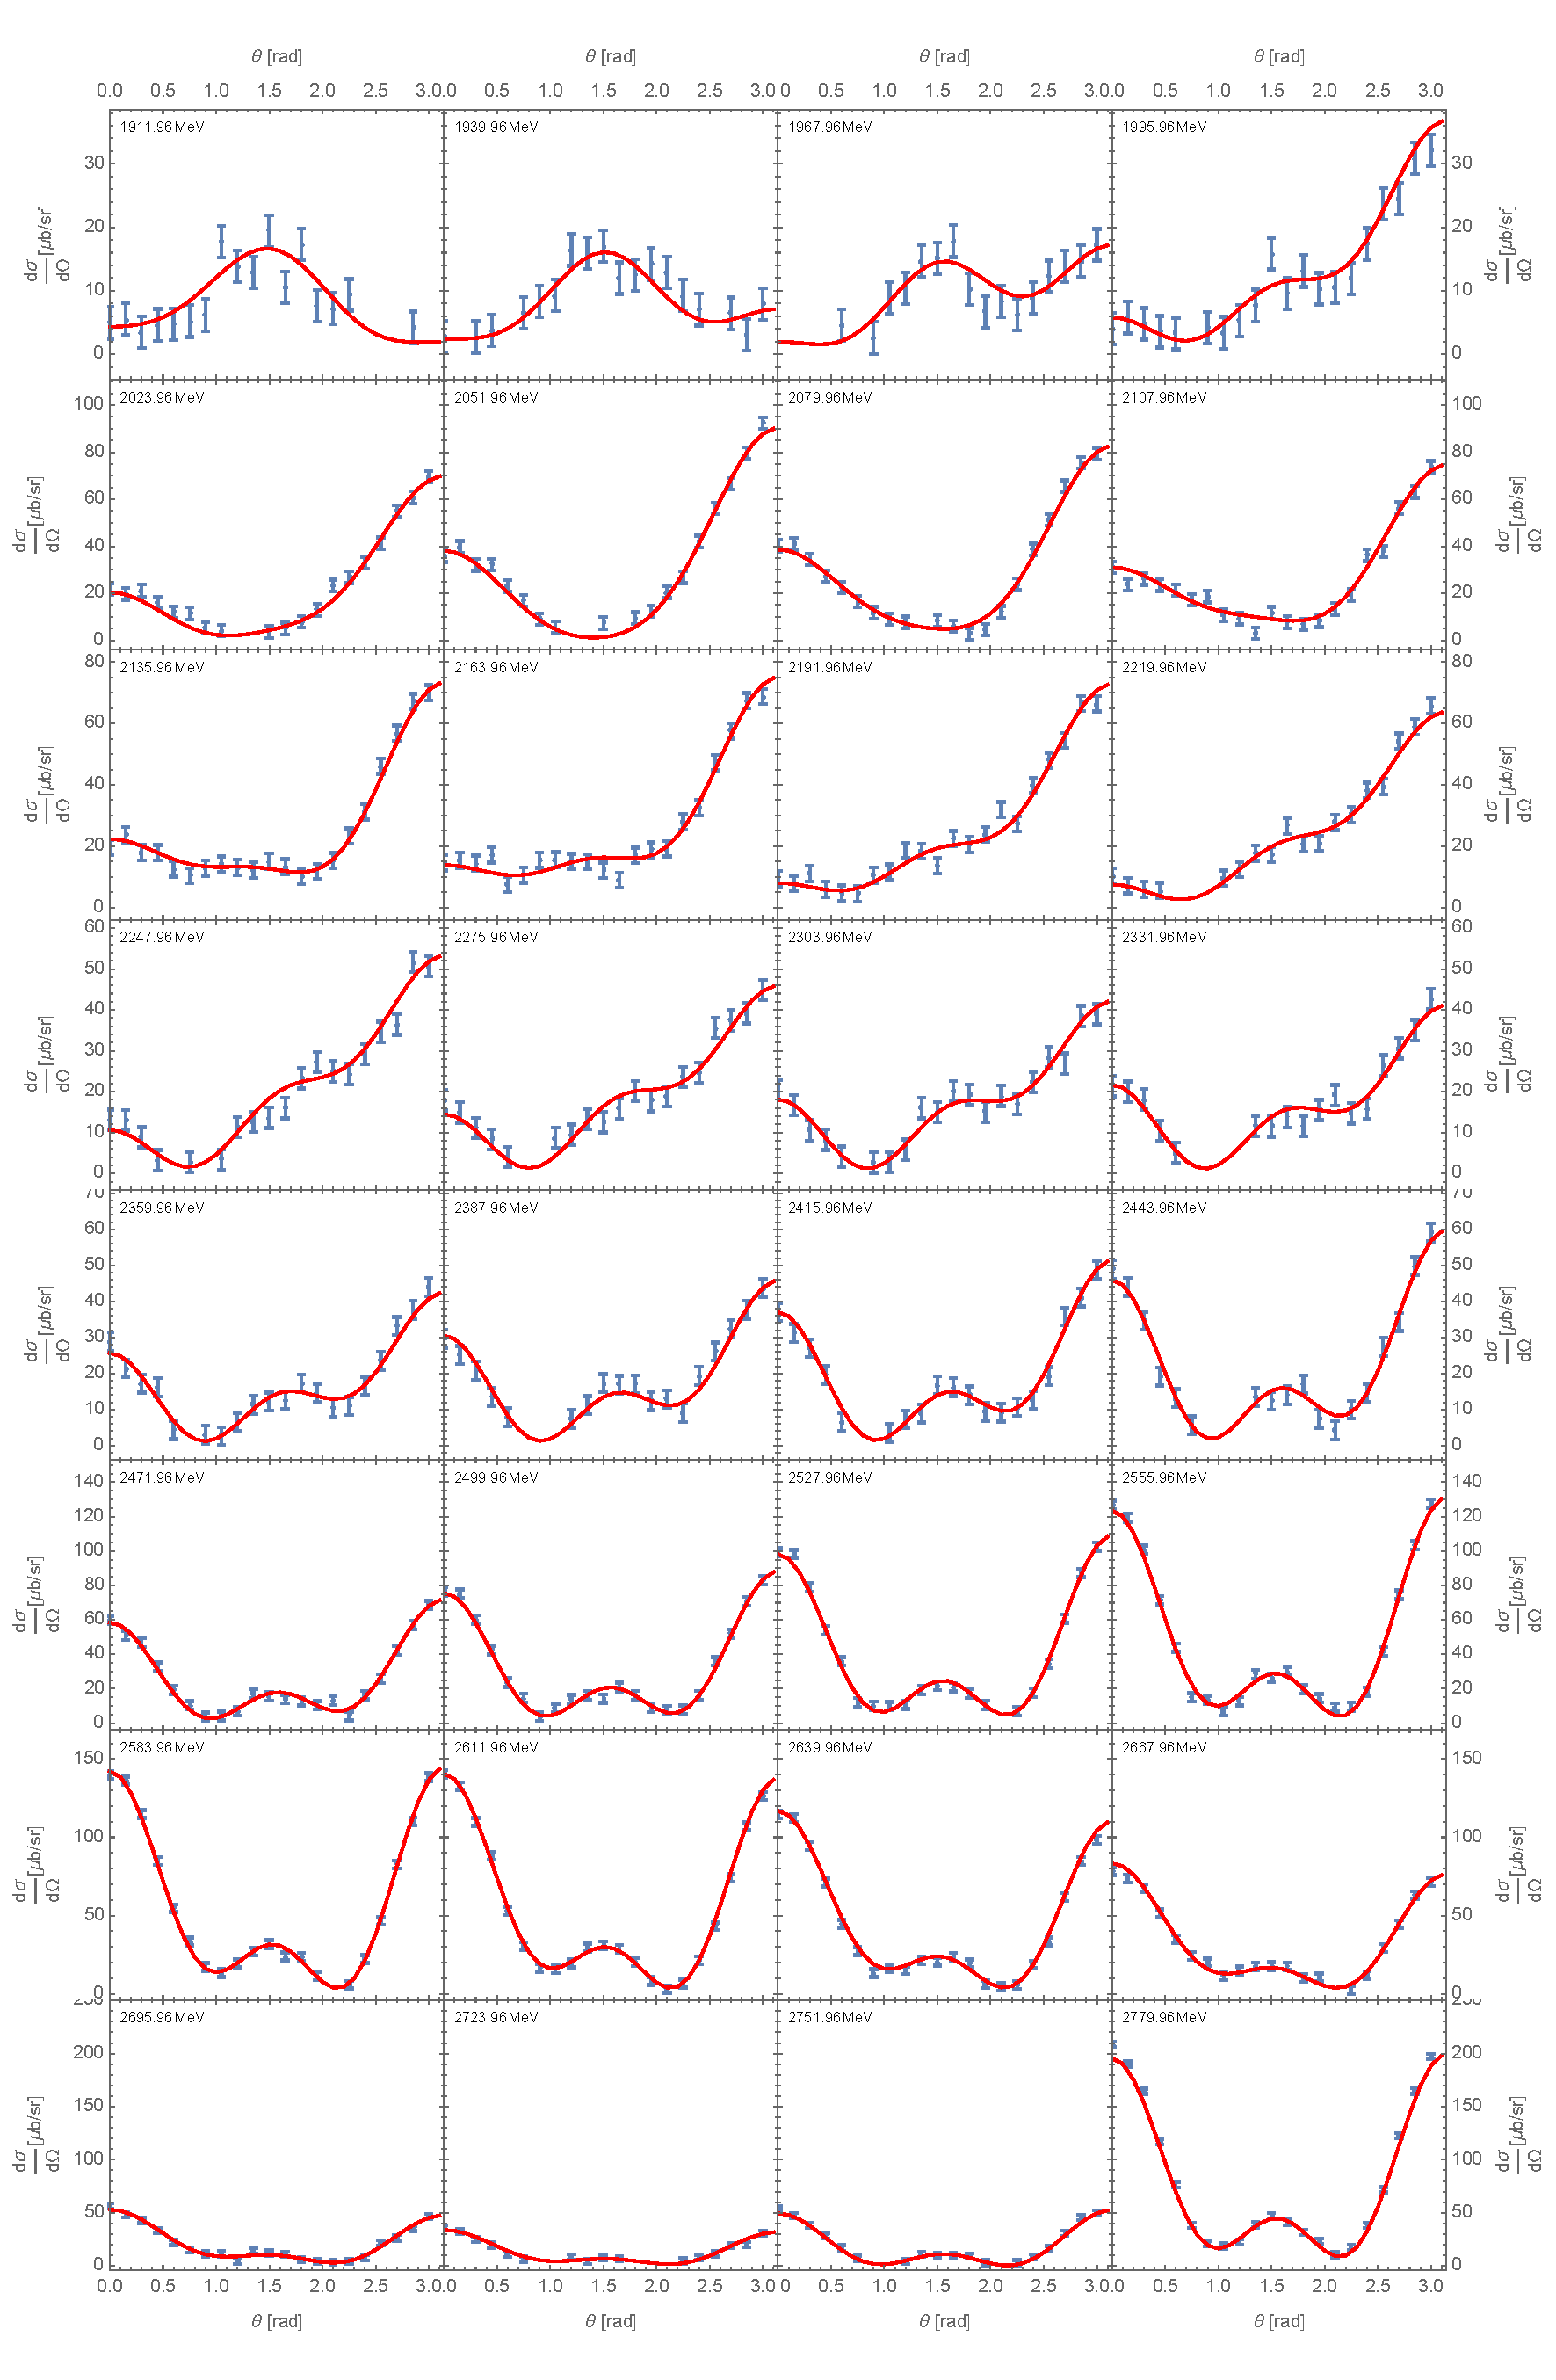
\includegraphics[width=0.49\linewidth,trim=0cm 0cm 1cm 7cm]{Diff2.pdf}\\
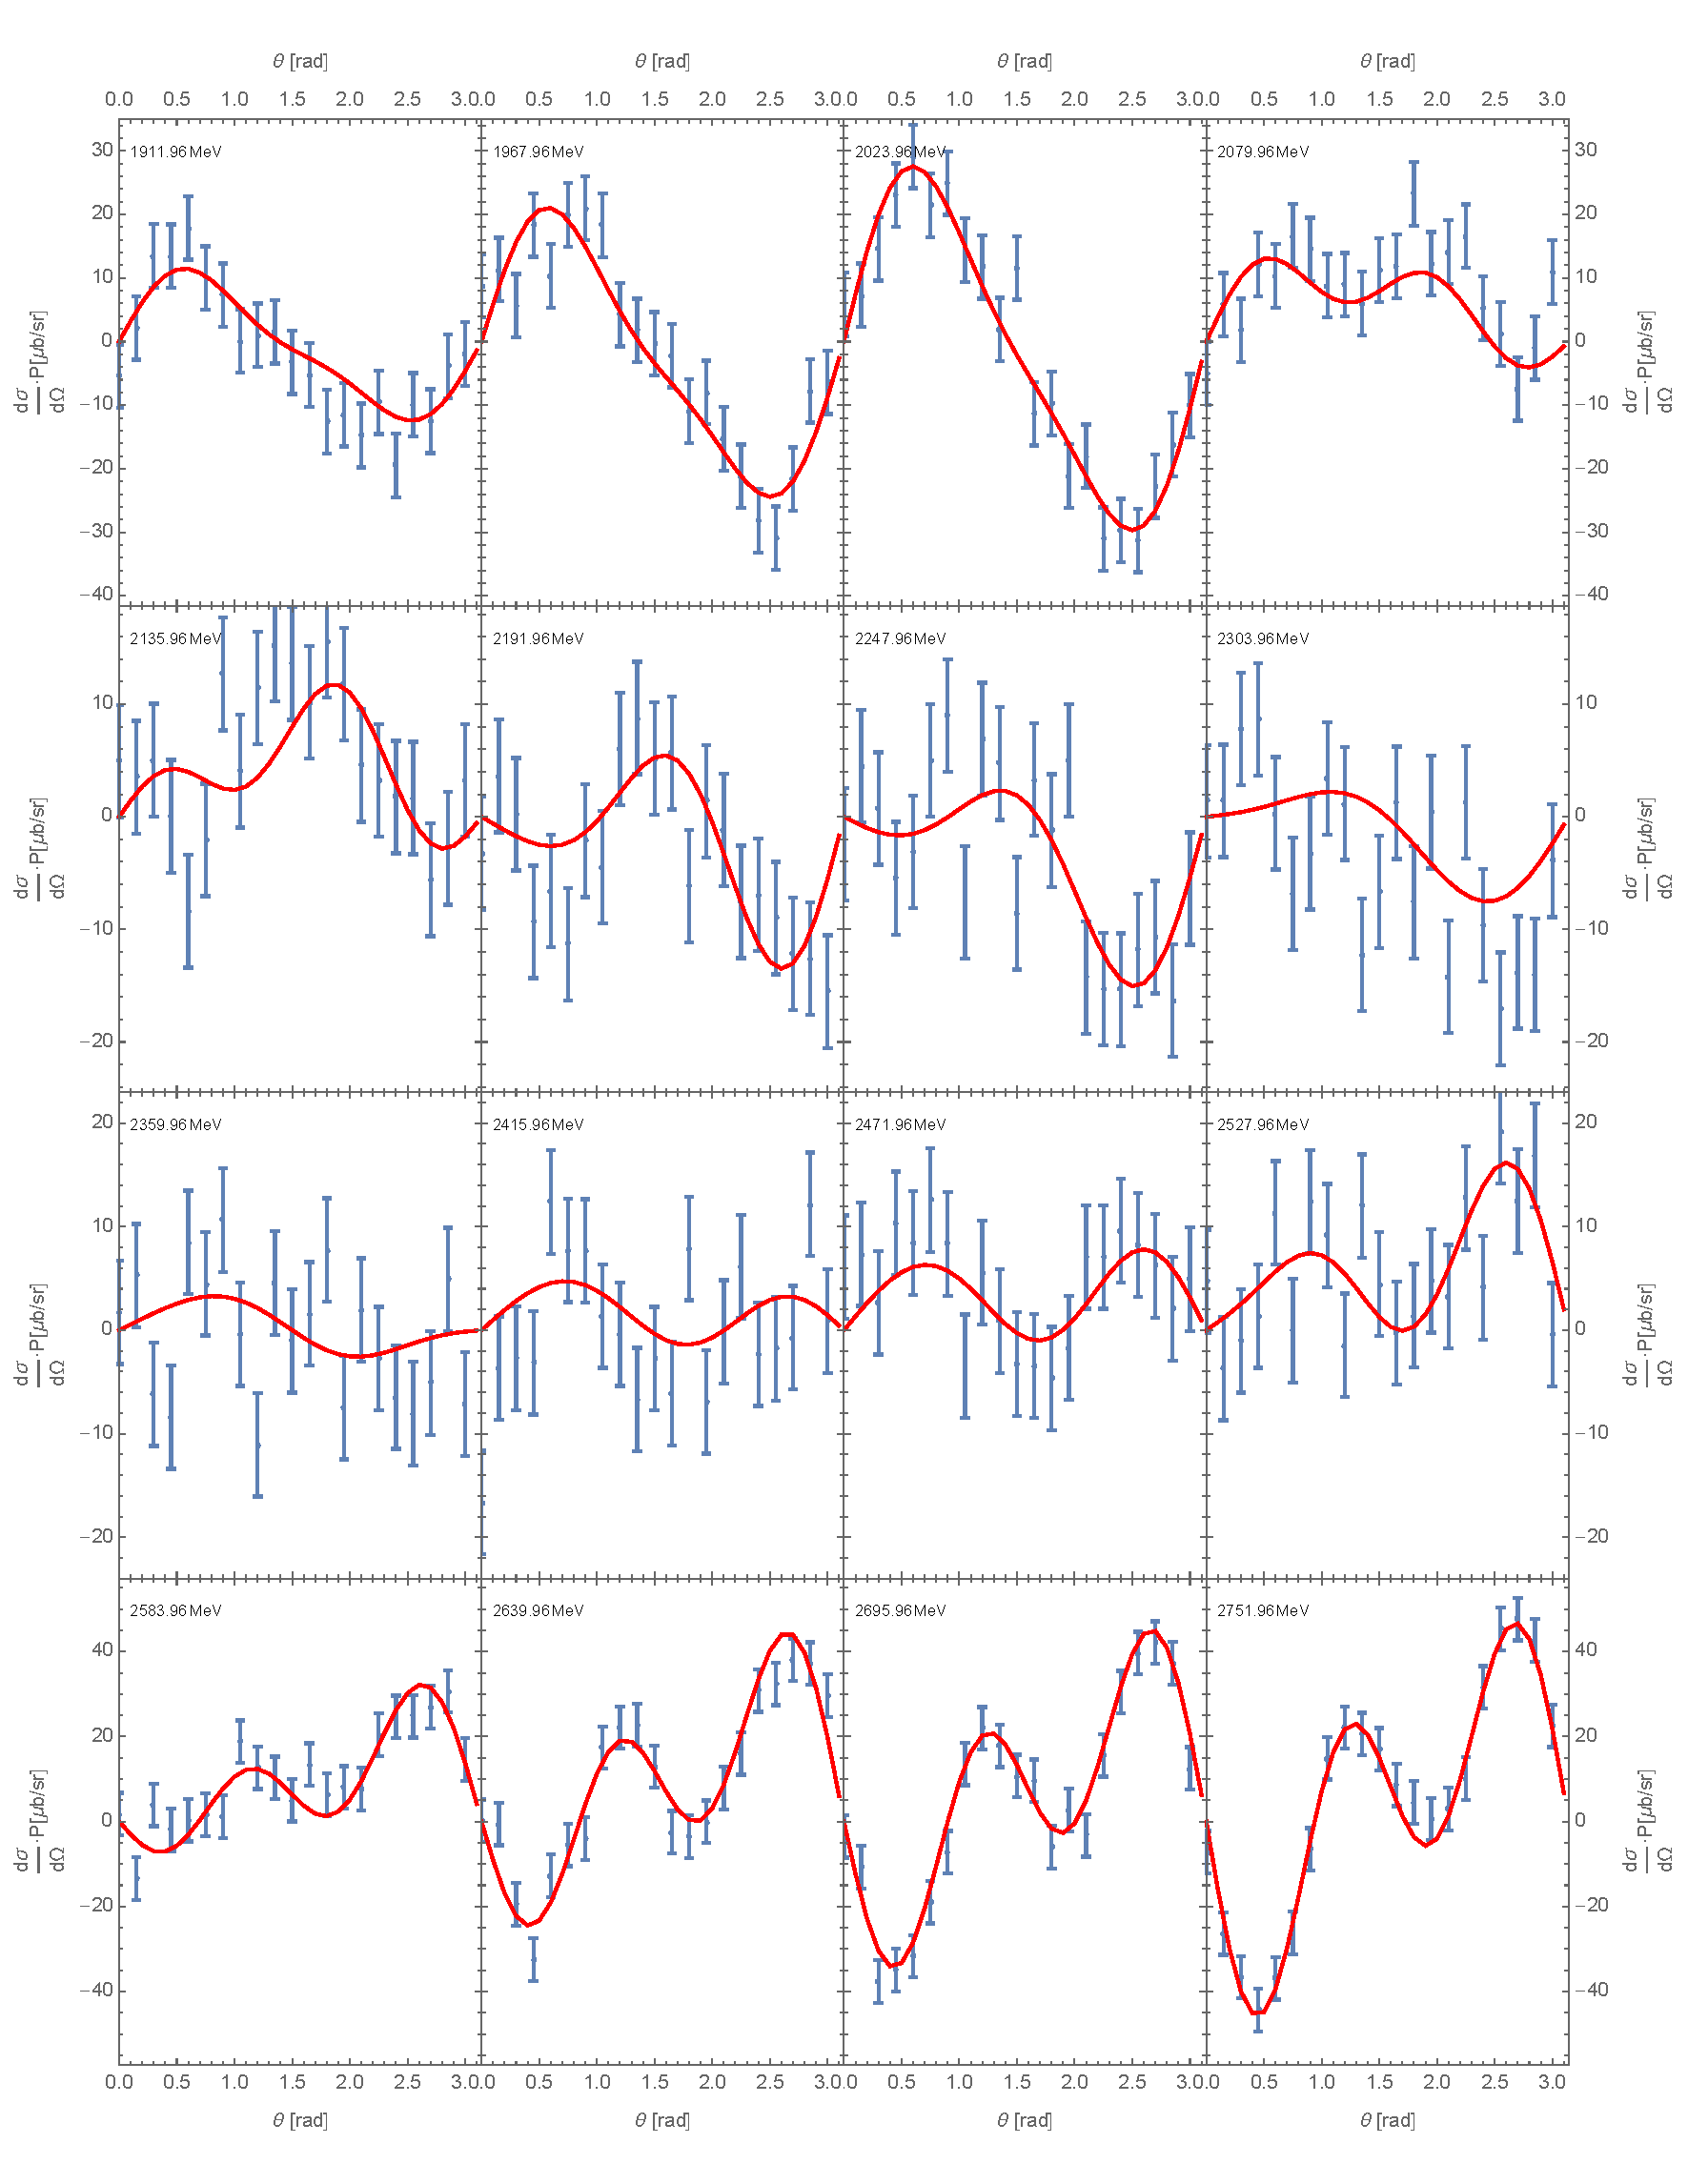
\includegraphics[width=0.49\linewidth,trim=1cm 1cm 0cm 0.5cm]{pol1.pdf}
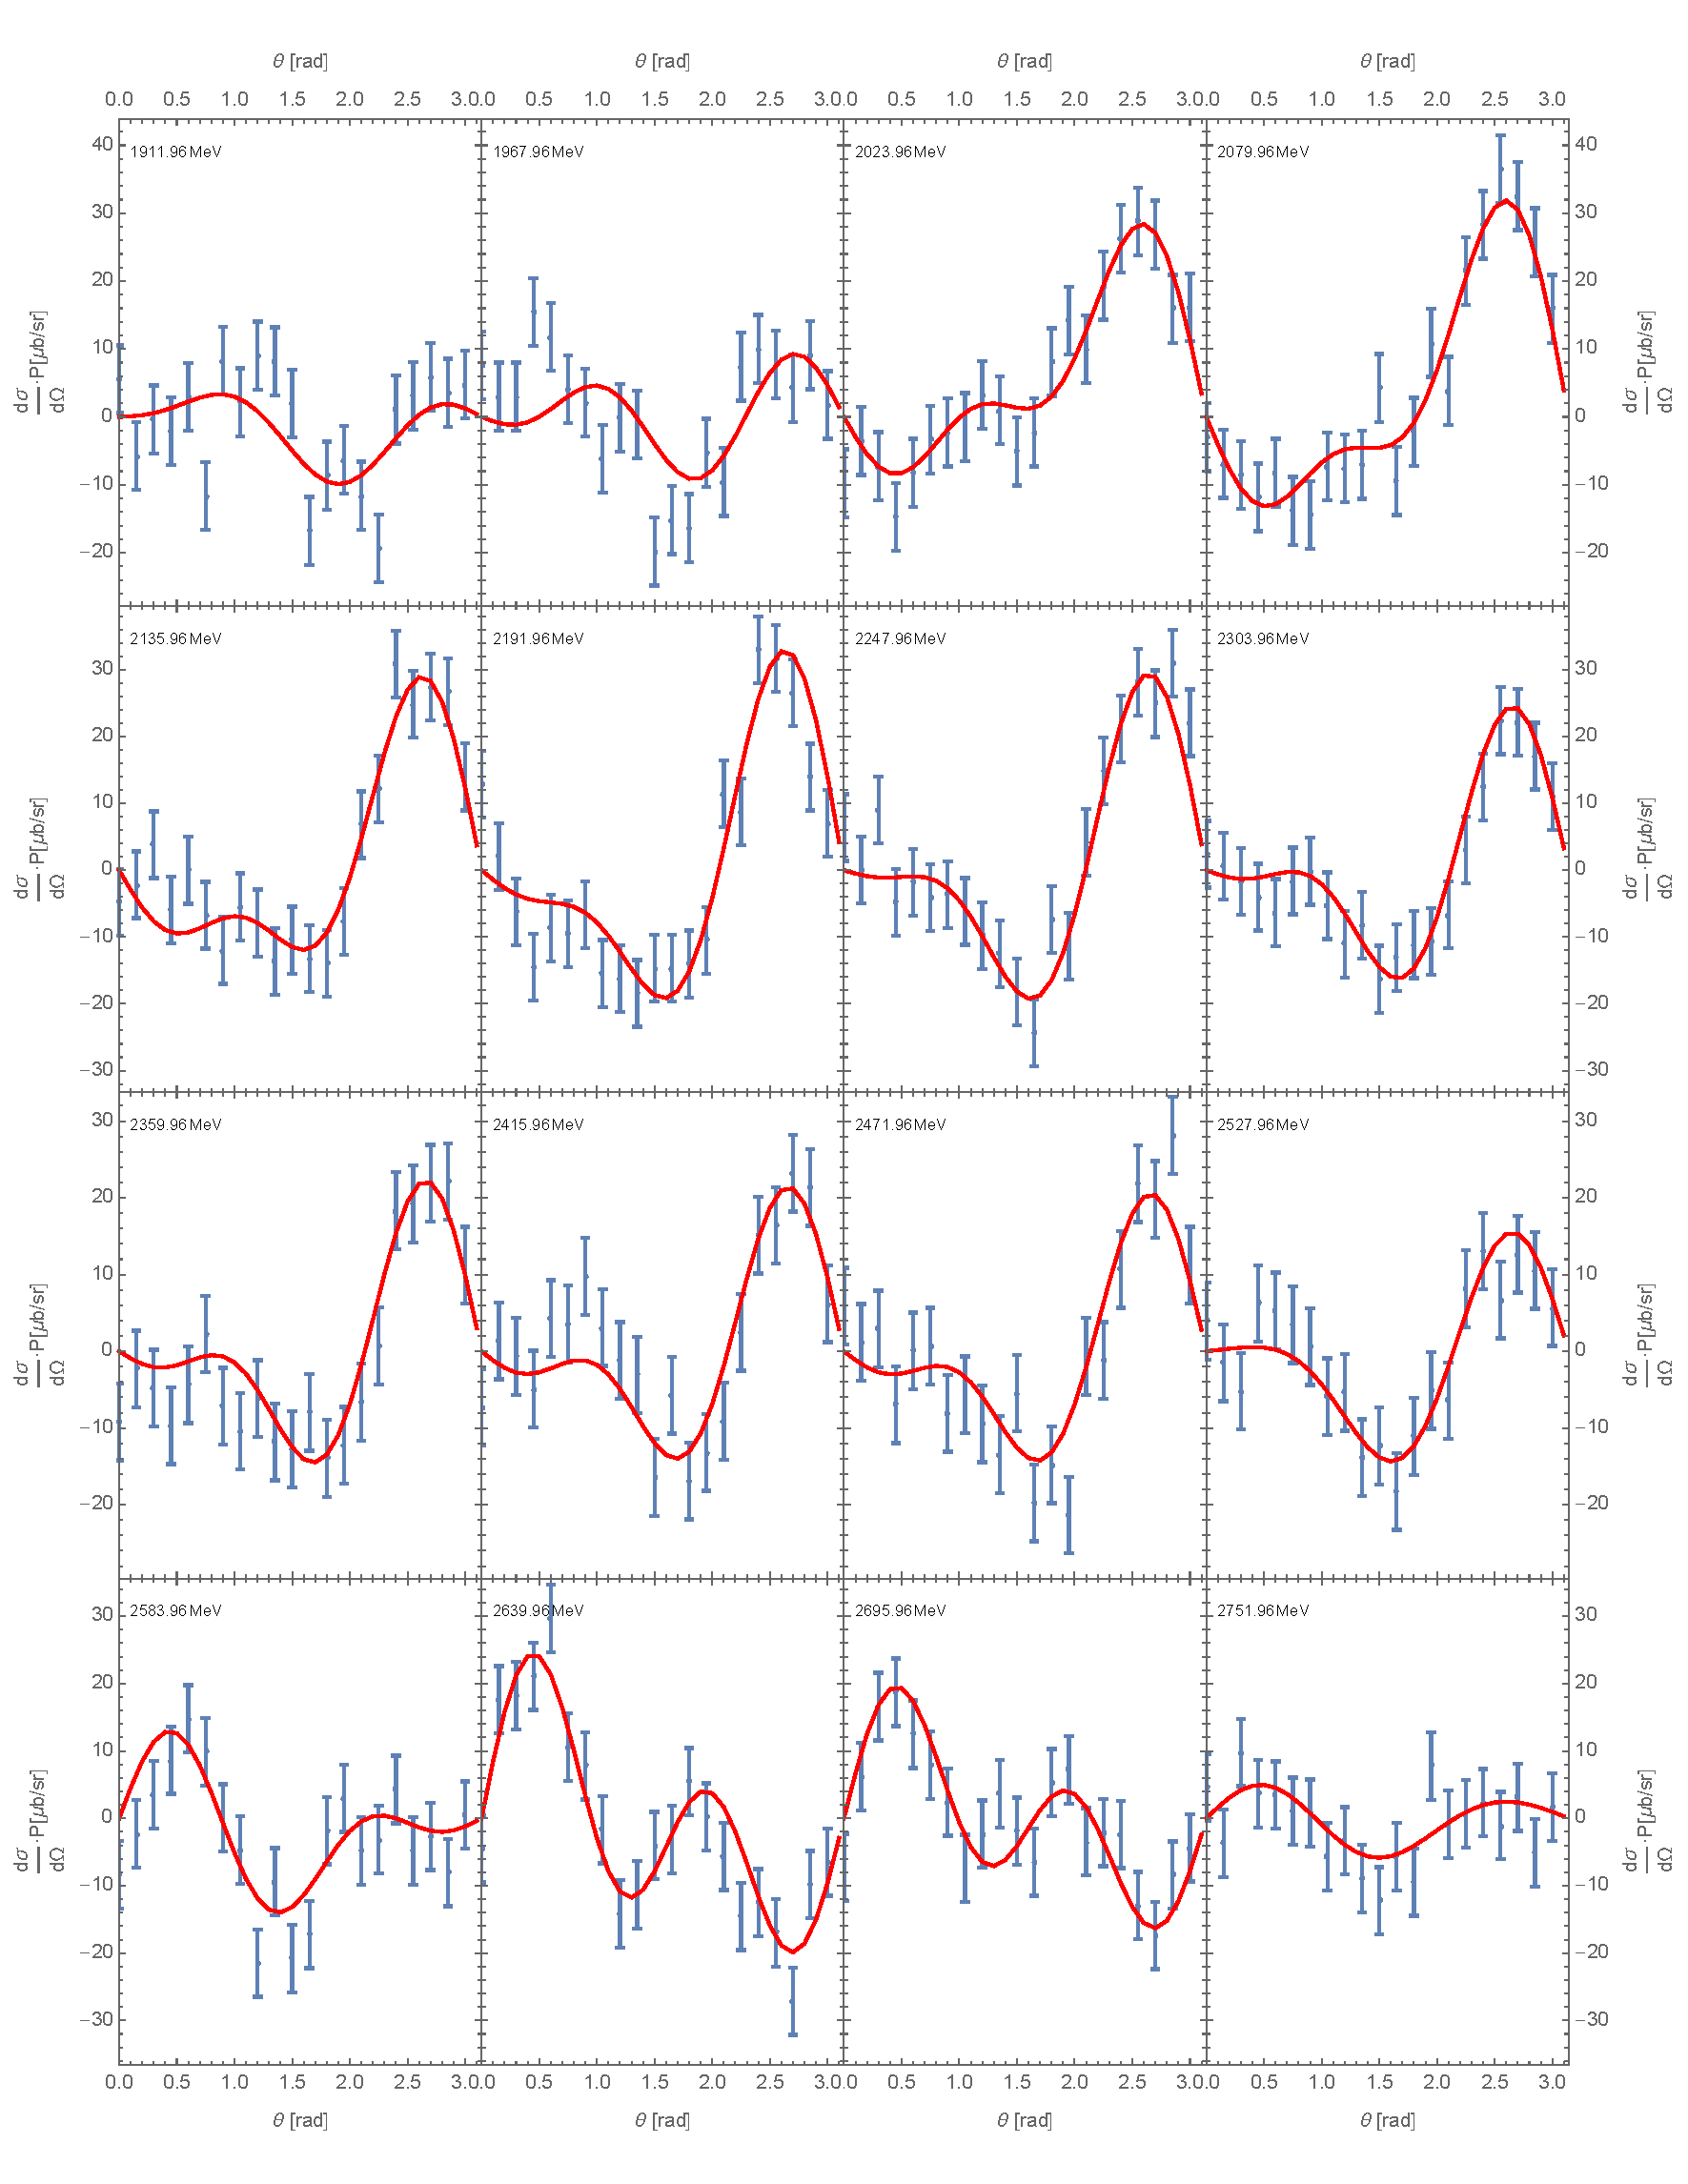
\includegraphics[width=0.49\linewidth,trim=0cm 1cm 1cm 0.5cm]{pol2.pdf}
\end{center}
\caption{Synthetic data for the  differential cross section and polarization in blue for the generating function in red.}
\label{fig:Fig3}
\end{figure}


\newpage
%%%%%%%%%%%%%%%%%%%%%%%%%%%%%%%%%%%%%%%%%%%%%%%
\section{Toy Model Fit Results} \label{sec:Toy Model Fit Results}


In later parts of the paper we discuss different implementations of the LASSO in detail on one particular dataset. Here, we describe some initial trials using those LASSO variants on three different datasets in order to get a robust understanding of the individual methods strengths and weaknesses before moving onto fitting the real data. The model used to generate all of the data sets was slightly more complicated than the model used to fit the data as noted in the introduction. All data sets were generated using the same contact parameters, energies, and error distributions; they differed with respect to the generation of resonances. Our main data set consisted of four resonances, each corresponding to a different partial wave with differing masses however we also looked at a data set containing four resonances all with the same mass as well as a set with two groups of two resonances in two different partial waves, all of differing masses. In our exploratory analysis, we found, as detailed later in the paper, that various implementations are more effective than others, however between datasets we found a consistency in which methods are better than others. It is for this reason that we move our discussion to the data set containing four resonances all of different masses, as it is the most general data set however our conclusions remain consistent across the other datasets. 

\subsection{Forward LASSO}

In this forward selection model, we are penalizing the occurrence of resonances by minimizing  $\chi^2+P(\lambda), \text{ where } P(\lambda) =   \lambda^4 \sum_{i=0}^{9}  |x_i|$. We run LASSO from $\lambda = 10 \text{ to } \lambda = 0$ decreasing in half integer steps. For a new step in $\lambda$, the converged solution for the next higher $\lambda$ is taken as start value. In other words, resonances are added until they are all present in the fit, at $\lambda=0$. From the BIC we see the minimum and thus our best model occurs at $\lambda=4$. This model contains 5 resonances, the 4 correct ones and 1 false one as indicated by Fig.~\ref{fig:Fig4}. Another indication of this being our best model comes from Pearson's $\chi^2$ test. All of the models from $\lambda=0$ to $\lambda=4$ pass Pearson's $\chi^2$ test for 95\% confidence.


\begin{figure*}
\begin{center}
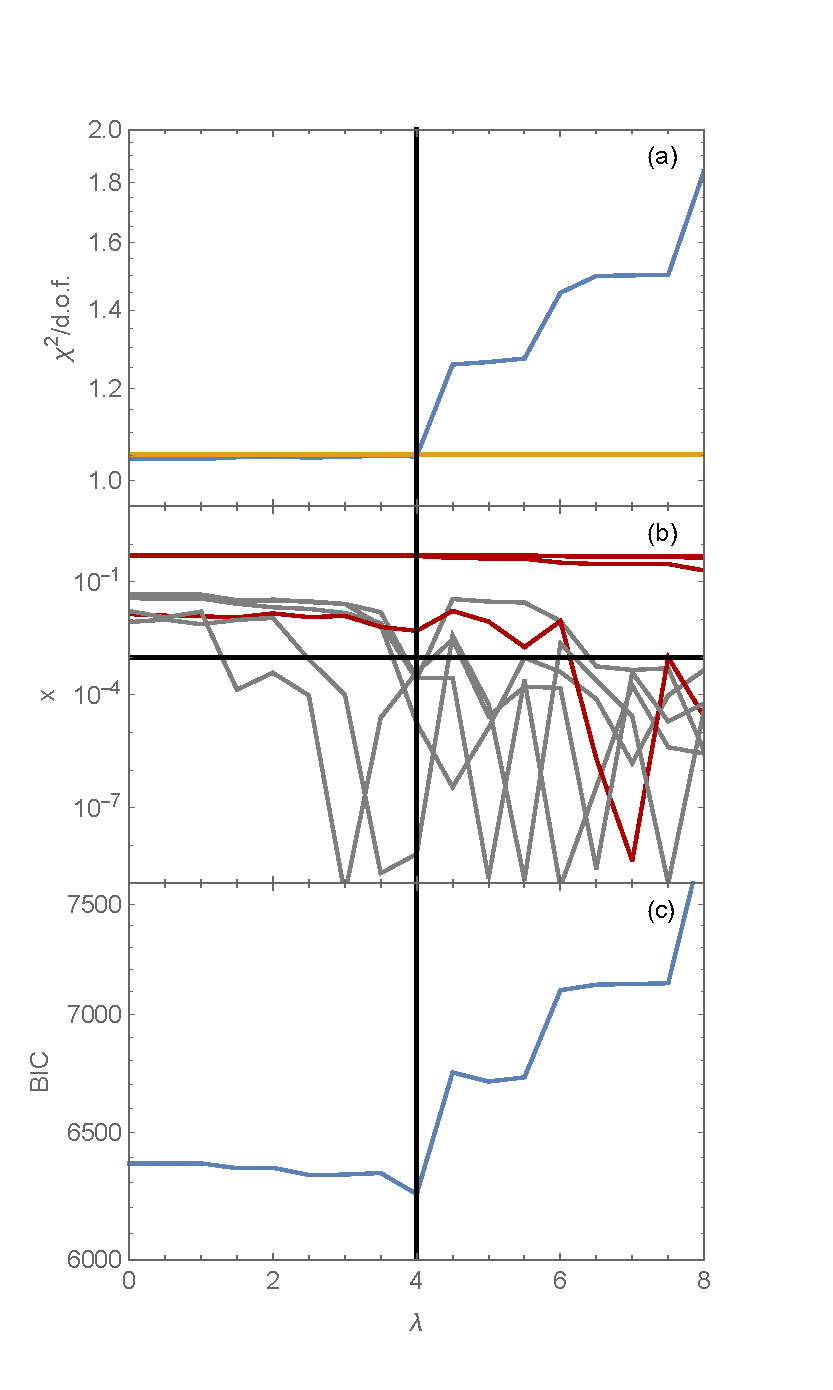
\includegraphics[width=.49\linewidth,trim=0 1cm 0 3cm]{Fig4a.pdf}
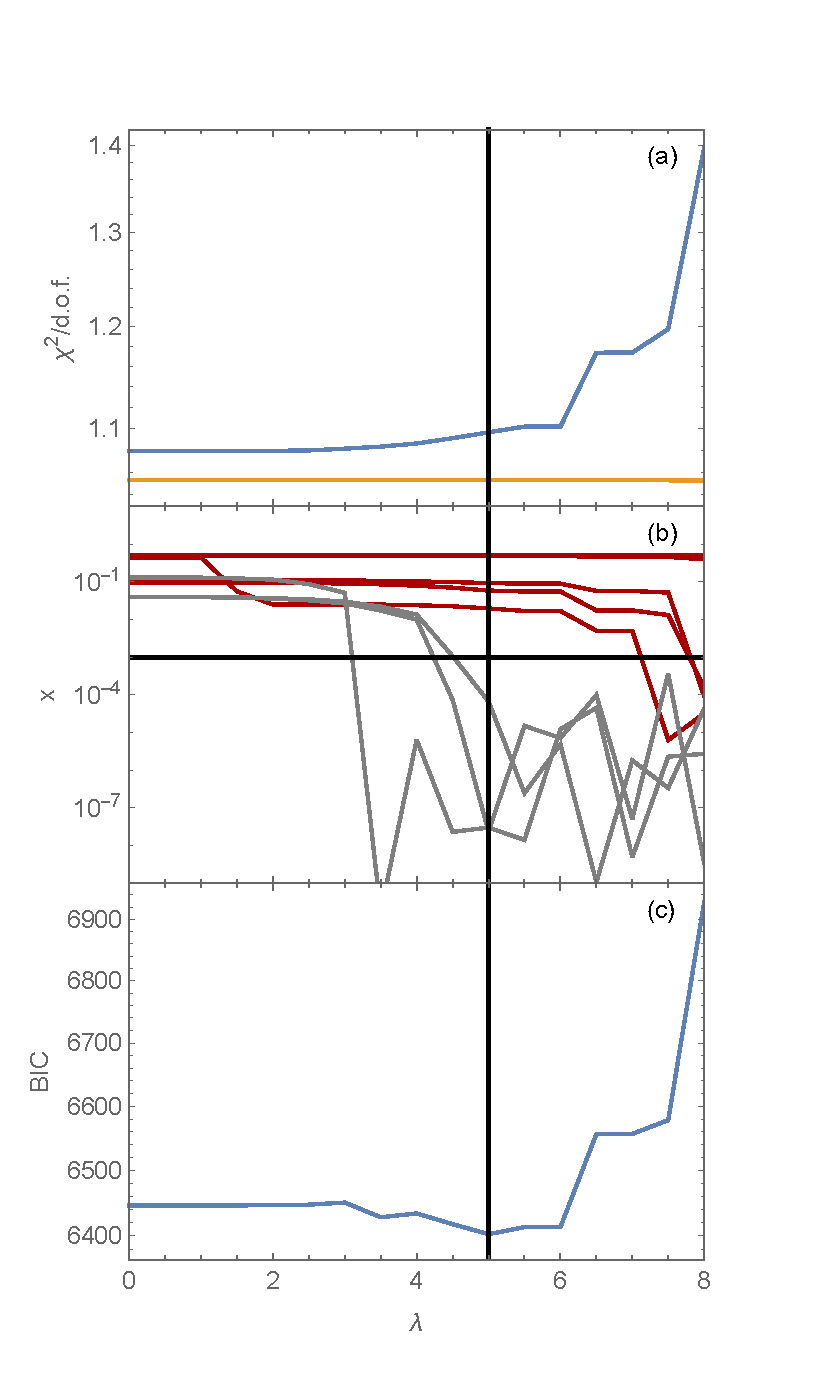
\includegraphics[width=.49\linewidth,trim=0 1cm 0 3cm]{Fig4b.pdf}
\caption{Fit results from forward (left) and backward (right) LASSO for the toy model. (a) $\chi^2$ per degree of freedom in blue with the Pearson's $\chi^2$ test per degree of freedom in orange, both as a function of $\lambda$.(b) Absolute value of the resonance amplitudes $x[i]$ as function of $\lambda$ in a logarithmic scale. Index $i$ denotes the corresponding partial wave indices $(I,J,L)$. The red lines indicate the finally chosen parameters, the gray lines show the unnecessary parameters. (c) The Bayesian Information Criterion (BIC).The vertical line signifies the minimum of the BIC and the chosen model.}
\label{fig:Fig4}
\end{center}
\end{figure*}

\subsection{Backward LASSO}

In this backwards selection model, we are penalizing the occurrence of resonances by minimizing  $\chi^2+P(\lambda), \text{ where } P(\lambda) =   \lambda^4 \sum_{i=0}^{9}  |x_i|   \text{. We run LASSO from } \lambda = 0 \text{ to } \lambda = 10$ increasing in half integer steps. From the BIC we see the minimum and thus our best model occurs at $\lambda=5$. This model contains 7 resonances, the 4 correct ones and 3 false ones as indicated by Fig.~\ref{fig:Fig4}. While there is a pronounced minimum in the BIC, this model fails Pearson's $\chi^2$ test for all values of $\lambda$ for 95\% confidence.

We interpret this as follows: In the backward LASSO, the fit allows for all resonances in the first optimization at $\lambda=0$. Apparently, a worse local minimum is found than in the forward LASSO, and increasing $\lambda$ does not help to escape that worse local minimum. In contrast, the forward LASSO starts with a very small number of resonances at high $\lambda$. In that lower-dimensional parameter space, only the most important resonances are allowed and a better local minimum can be found. Forward LASSO is therefore in general preferable to backward LASSO (in linear regression there obviously no difference because there is only one local minimum).

\begin{figure*}
\begin{center}
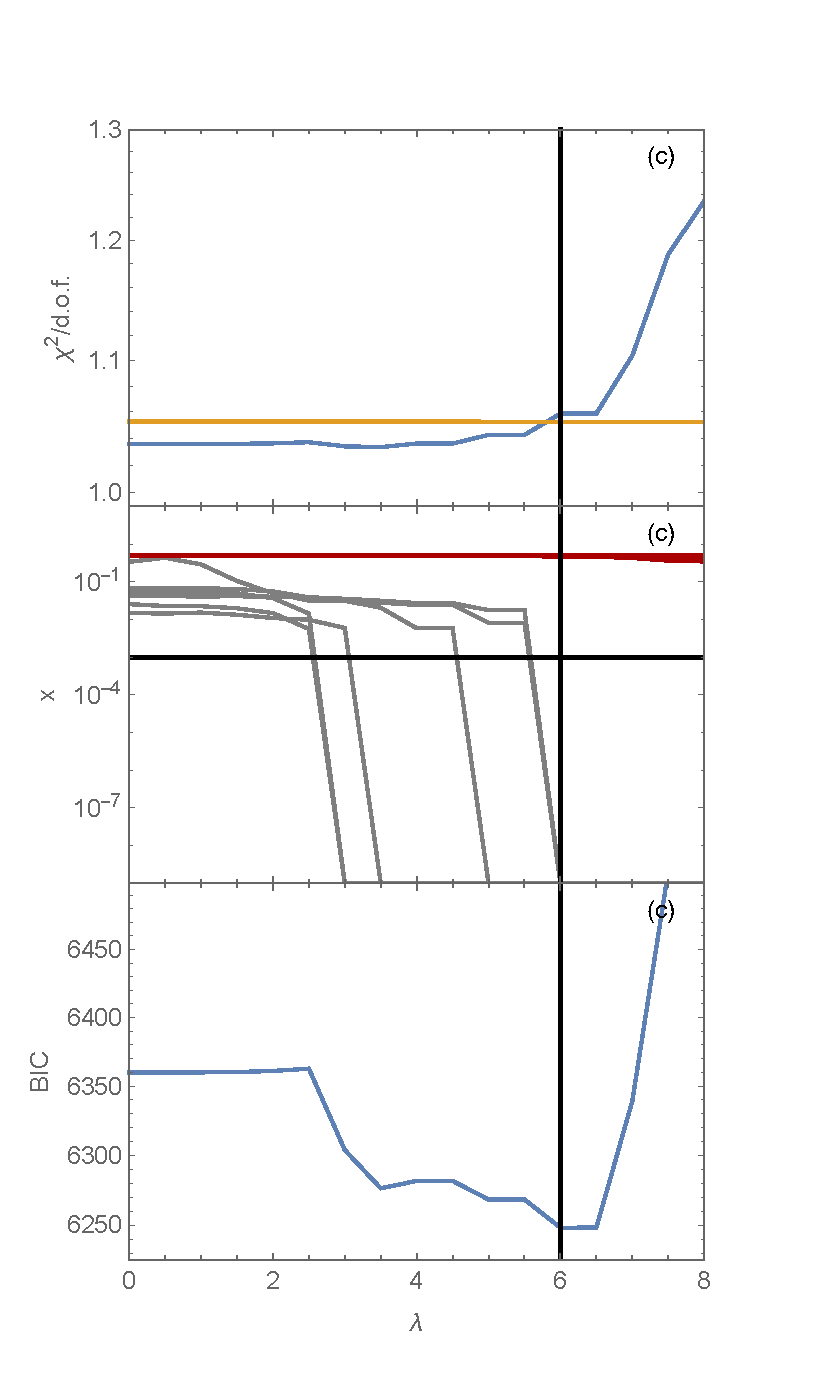
\includegraphics[width=.49\linewidth,trim=0 1cm 0 3cm]{Fig5a.pdf}
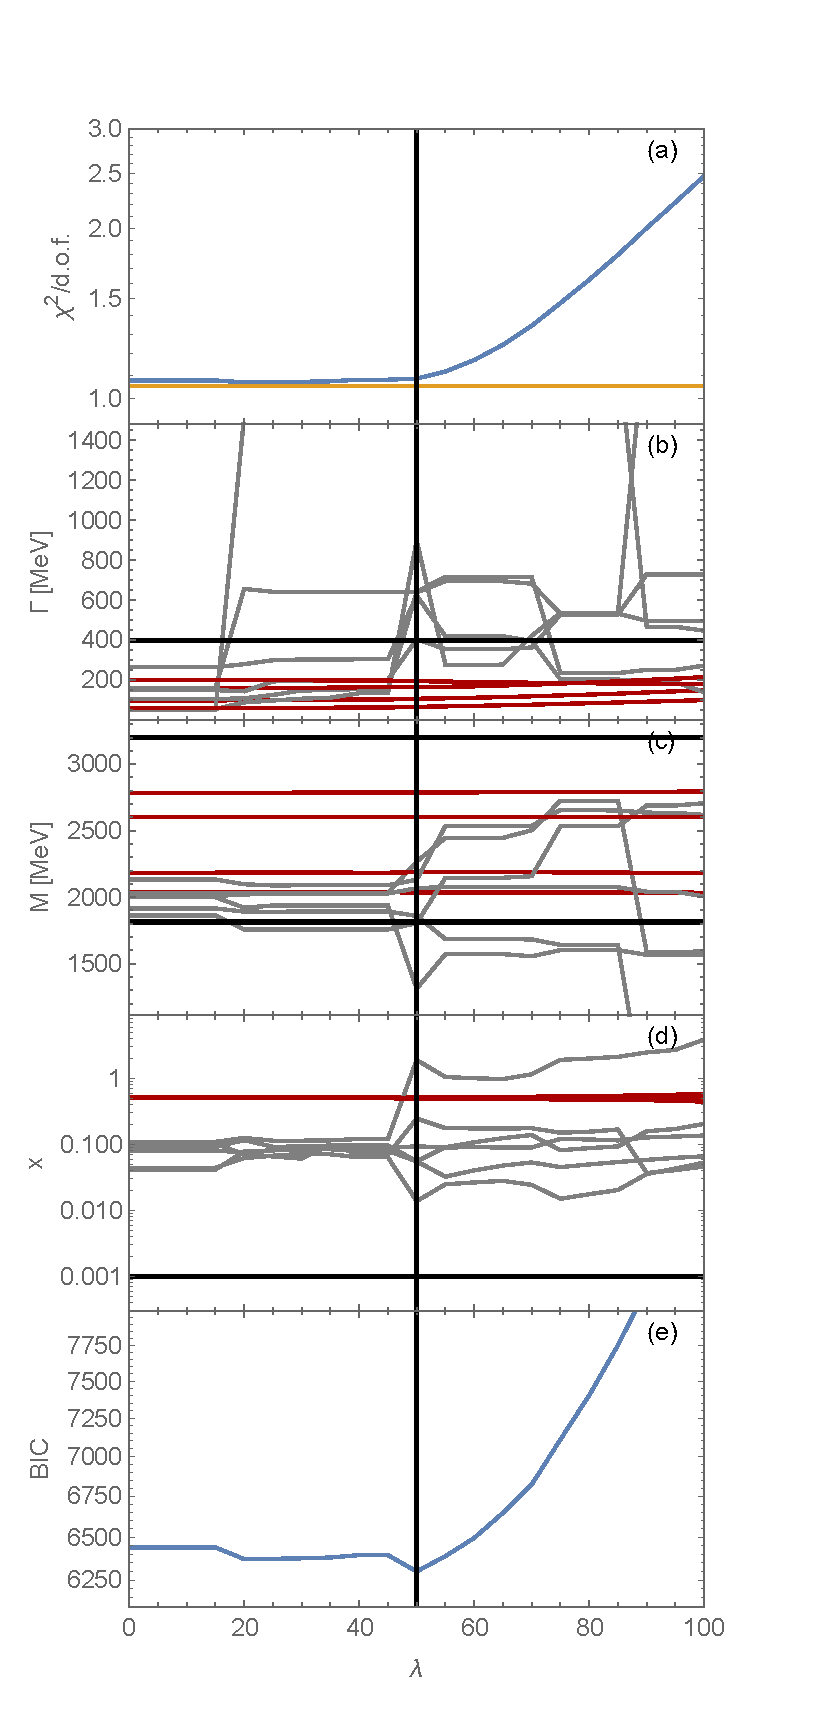
\includegraphics[width=.49\linewidth,trim=0 1cm 0 3cm]{Fig5b.pdf}
\caption{Fit results from Backwards Automatic Shutoff LASSO (left) and forwards LASSO with Second Derivative Penalty (right). For the Backwards Automatic Shutoff (a) $\chi^2$ per degree of freedom in blue with the Pearson's $\chi^2$ test per degree of freedom in orange, both as a function of $\lambda$. (b) Absolute value of the resonance amplitudes $x[i]$ as function of $\lambda$ in a logarithmic scale. The red lines indicate the finally chosen parameters, the gray lines show the unnecessary parameters. (c) The Bayesian Information Criterion (BIC). The vertical line signifies the minimum of the BIC and the chosen model.
Right: For the penalty of the second derivative (a) $\chi^2$ per degree of freedom in blue with the Pearson's $\chi^2$ test per degree of freedom in orange, both as a function of $\lambda$. (b) The resonance width $\Gamma[i]$ as function of $\lambda$ in a logarithmic scale.(c) The resonance mass $M[i]$ as function of $\lambda$ in a logarithmic scale.(d) The resonance amplitude $x[i]$ as function of $\lambda$ in a logarithmic scale. Index $i$ denotes the corresponding partial wave indices $(I,J,L)$. The red lines indicate the finally chosen parameters, the gray lines show the unnecessary parameters. (e) The Bayesian Information Criterion (BIC). The vertical line signifies the minimum of the BIC and the chosen model.}
\label{fig:Fig5}
\end{center}
\end{figure*}

\subsection{Backward Automatic Shutoff LASSO}

Our Backwards Automatic Shutoff LASSO method is a greedier modification of our Backward LASSO. We are still penalizing the occurrence of resonances by minimizing  $\chi^2+P(\lambda), \text{ where } P(\lambda) =   \lambda^4 \sum_{i=0}^{9}  |x_i|   \text{as we iterate LASSO from } \lambda = 0 \text{ to } \lambda = 10$ increasing in half integer steps. The modification is that once a resonance amplitude ($x$) becomes smaller than $10^{-3}$, which is our zero, that resonance parameter is permanently removed from the model and is no longer fit for the remaining iterations. From the BIC we see the minimum and thus our best model occurs at $\lambda=6$. This model contains only the 4 real resonances, successfully sending all of the others to zero as seen in Fig.~\ref{fig:Fig5}. The minimum in the BIC also corresponds with with the intersection of the $\chi^2$ and the value given from Pearson's $\chi^2$ test  for 95\% confidence indicating that the model passes the test.




\subsection{Second Derivative Penalty}

In this modification of backwards selection, we follow the same procedure as the normal backwards LASSO except the penalty term $P(\lambda)$ is calculated by integrating from threshold to the maximum fitted energy the modulus squared of second derivative of the resonance and then normalized by dividing by the integral of the modulus squared of the resonance. Analytically $P(\lambda)$ is expressed as the following.
%\begin{eqnarray}
%P(\lambda)= \lambda^5 \sum_{i=0}^{\text{9}} \frac{8 \left( \frac{2(W-M[i])\Gamma[i](12 M[i]^2 -24 M[i] W +12 W[i]^2 +5 \Gamma[i]^2)}{(4M[i]^2-8M[i]W +4W^2+\Gamma[i]^2)^2} + 3 \arctan{\frac{2(W-M[i])}{\Gamma[i]}} \right)}{\Gamma[i]^4 \arctan{\frac{2(W-M[i])}{\Gamma[i]}}}\,,
%\end{eqnarray}
\begin{widetext}
\begin{eqnarray}
P(\lambda)= \lambda^5\sum_{i=0}^{\text{9}} \int_{m_K+m_{\Xi}}^{3200} \frac{\partial^2}{\partial W^2} \left( | -x_i\,e^{i\Phi_i} \frac{\Gamma_i}{2(W-M_i+i \frac{\Gamma_i}{2})}|^2 \right) dW\,,
\end{eqnarray}
\end{widetext}
where index $i$ denotes the corresponding partial wave indices $(I,J,L)$. 
This penalty term is significantly different than the normal penalty of just the resonance amplitude $x$ since this penalty term depends only on $\Gamma$ and $M$. This allows for resonances effectively disappearing by their widths becoming too large that they flatten out and become essentially background or by their masses moving outside of the fitted region. The fit results can be seen in Fig.~\ref{fig:Fig5}. A 3D visualization of the penalty can be seen in  Fig.~\ref{fig:Fig6}. For our fit results, we chose our cutoff in width to be 400 MeV and our mass window to be 1813.29 (threshold) - 3200 (Highest fitted energy) MeV. Our fit results using this method were consistent with that of the automatic shut off. This method was able to correctly identity the four real resonances while eliminating the others by sending their widths above 400 MeV and their masses out of the fitted energy window.


\begin{figure}
\begin{center}
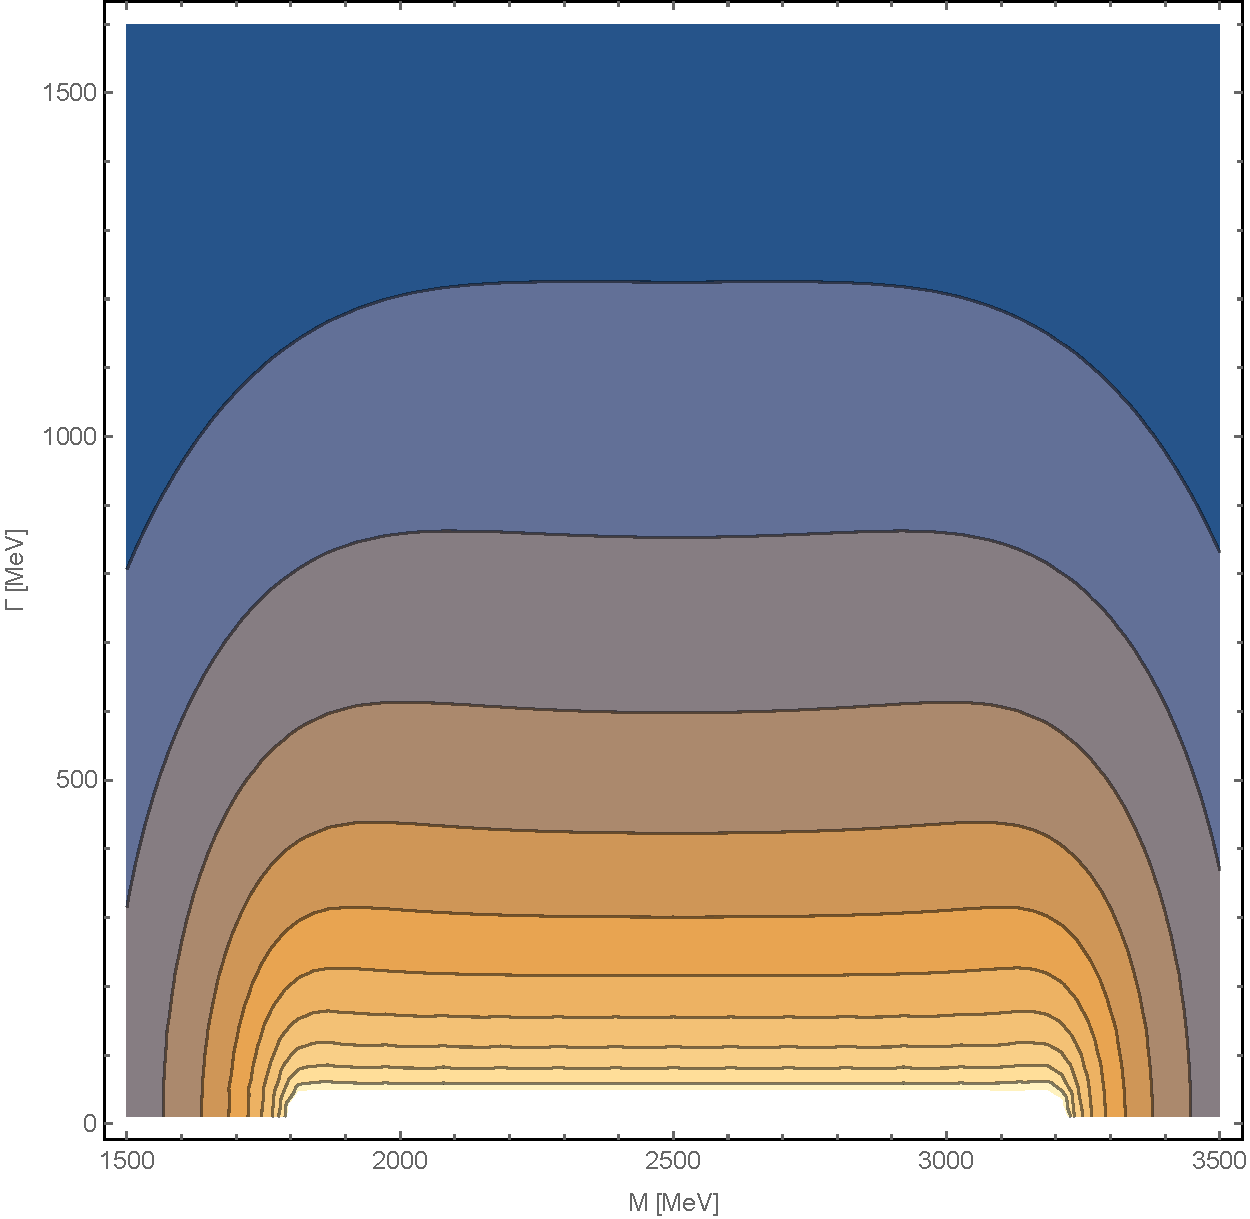
\includegraphics[width=0.99\linewidth]{Fig6A.pdf}
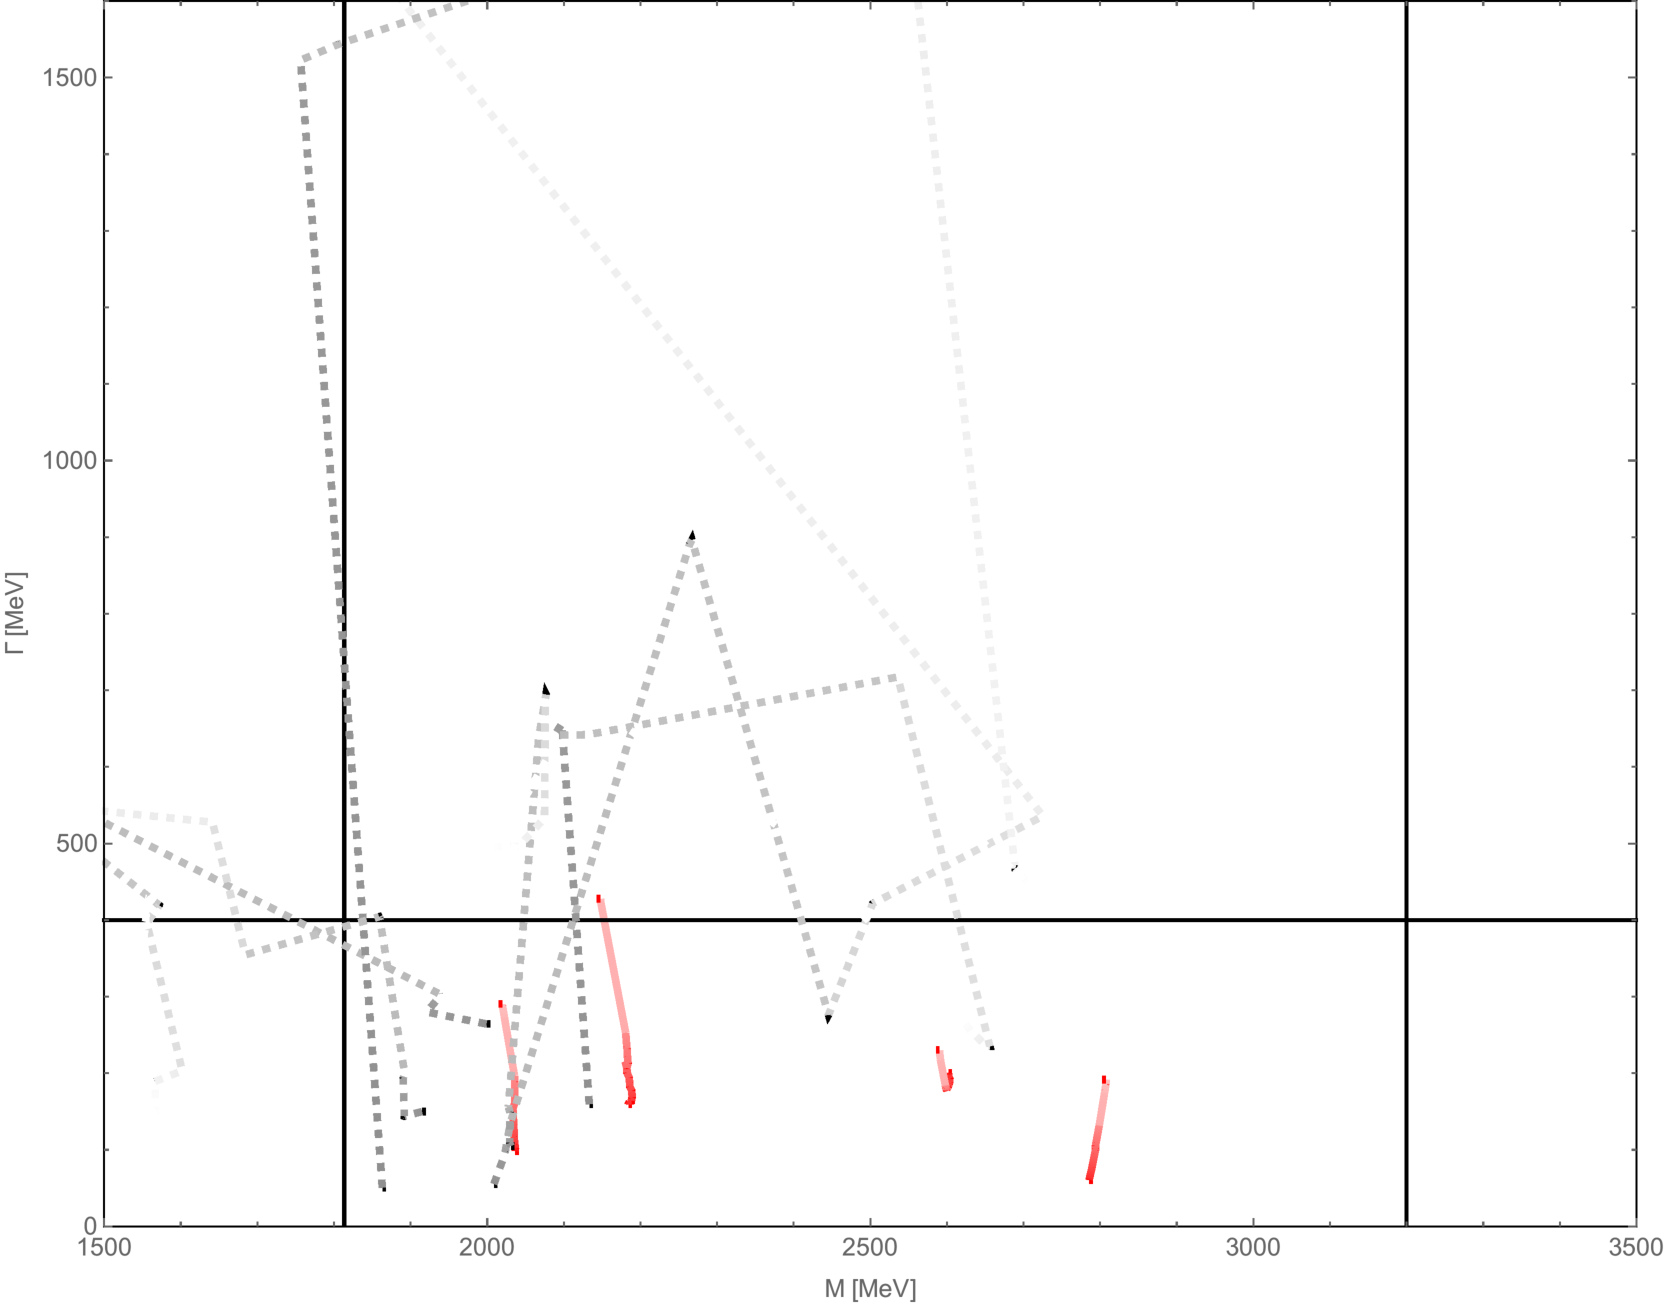
\includegraphics[width=0.99\linewidth]{fig6.pdf}
\caption{Left: Log-scale contour-plot of the penalty on the second derivative as a function of both mass M and width $\Gamma$. Right: Resonance mass and width $\Gamma$ from fit to toy model. Resonances in red are the real ones and resonances in gray are superfluous. The resonances fade in brightness as the tuning parameter $\lambda$ increases. The vertical lines signify the mass cut off window while the horizontal line signifies the width cut off at 400 MeV.
\com{Make figures same label size, label names, plot ranges; show trajectory for all lambda, and make big fat star at best lambda for all curves. Lower plot: Make all lines thicker, start with more intense black. Use more lambda to sample the trajectory and make it smoother. Upper figure: Take away the color coded bar on the right.}
}
\label{fig:Fig6}
\end{center}
\end{figure}


%%%
\section{Pruned Data Fit Results} \label{sec:Pruned Data Fit Results}


\subsection{Backward Automatic Shutoff LASSO}

Following the procedure laid out in section 2.3, our fit results for the real data can be seen in Fig.\ref{fig:Fig7}. From the BIC we see the minimum and thus our best model occurs at $\lambda=4.5$. This model contains only 1 resonance, sending all of the others to zero. For all models, the value from Pearson's $\chi^2$ test for 95\% confidence is larger than the real $\chi^2$ indicating that all of models passes the test.

\subsection{Second Derivative Penalty}

Following the procedure laid out in section 2.4, our fit results for the real data can be seen in Fig.\ref{fig:Fig7} and Fig.\ref{fig:Fig8}. From the BIC we see the minimum and thus our best model occurs at $\lambda=80$. This model contains only 1 resonance, sending all of the others to zero. For all models the $\chi^2_{d.o.f}$ is smaller than one and smaller than the value from Pearson's $\chi^2$ test for 95\% confidence indicating that the model passes the test as well as an over fit.
Unlike with the toy model, our results using this method were inconsistent with that of the automatic shut off. While both eliminated all but one resonance, the each method left one resonance with different quantum numbers than the other.




\begin{figure}
\begin{center}
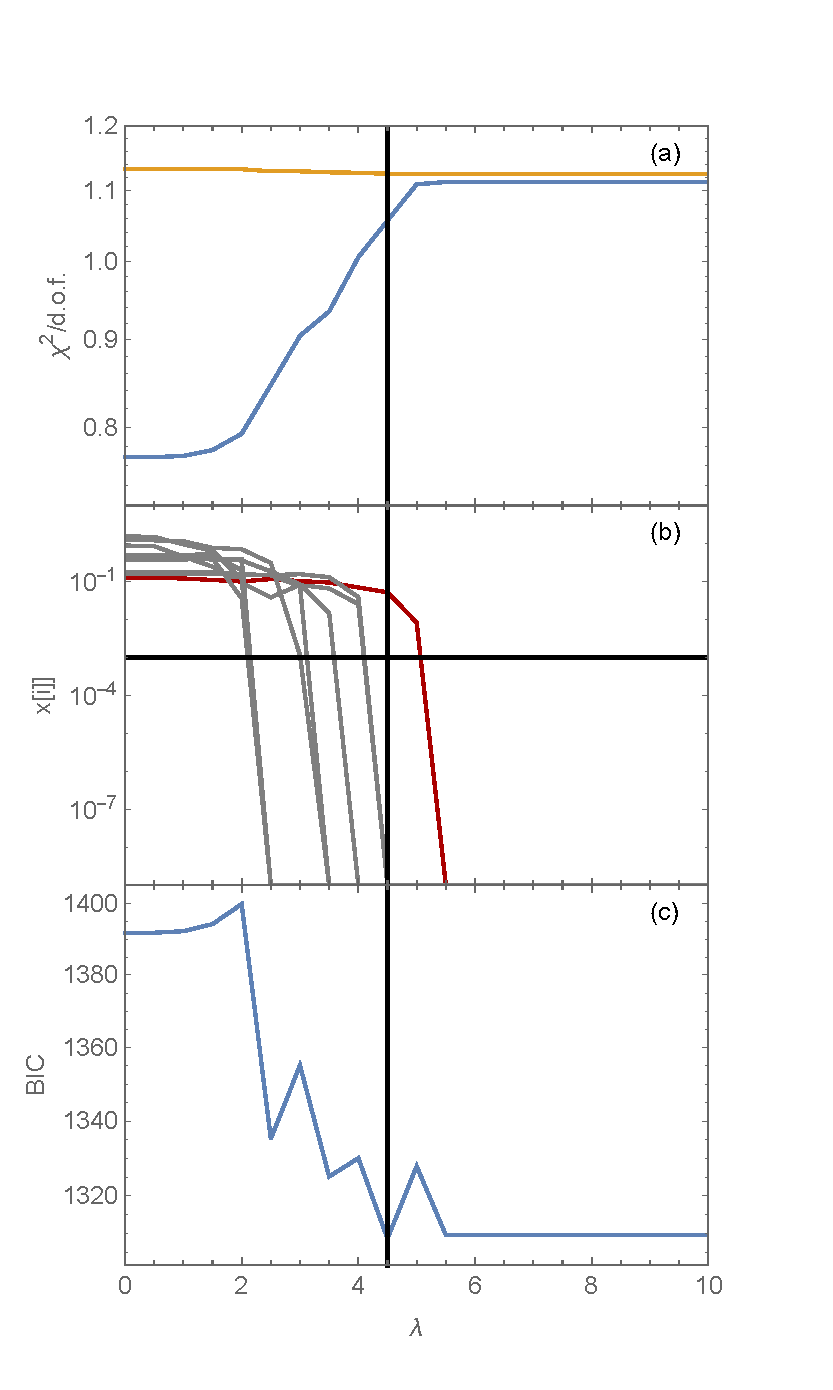
\includegraphics[width=.49\linewidth,trim=0 1cm 0 3cm]{Fig7.pdf}
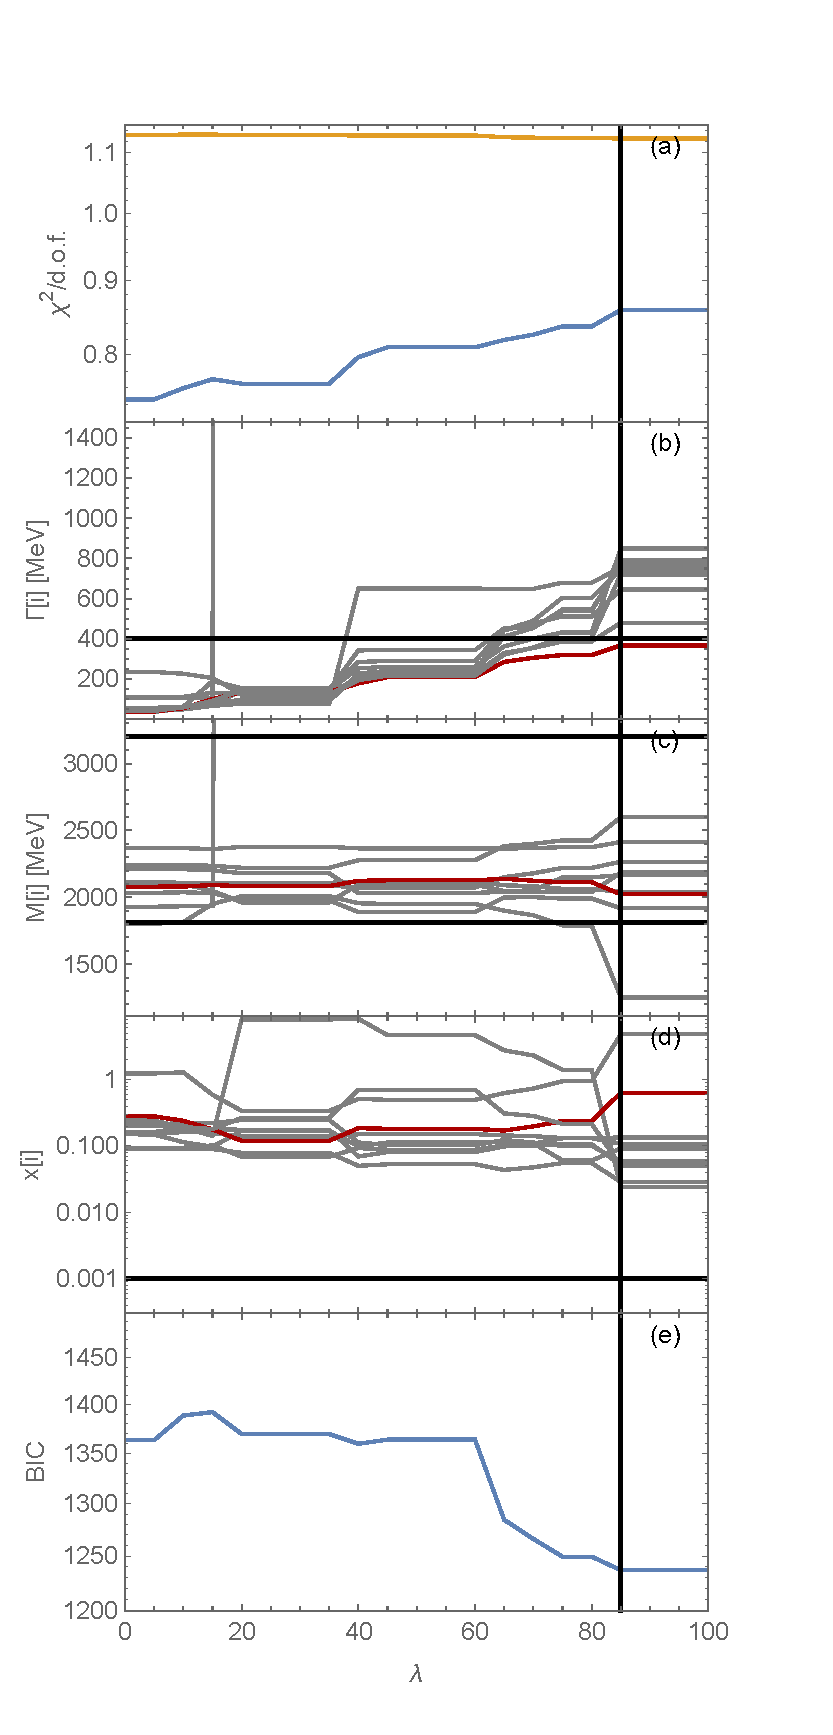
\includegraphics[width=.49\linewidth,trim=0 1cm 0 3cm]{Fig8A.pdf}
\caption{Left: Backwards Automatic Shutoff (a) $\chi^2$ per degree of freedom in blue with the Pearson's $\chi^2$ test per degree of freedom in orange, both as a function of $\lambda$. (b) Absolute value of the resonance amplitudes $x[i]$ as function of $\lambda$ in a logarithmic scale. The red lines indicate the finally chosen parameters, the gray lines show the unnecessary parameters. (c) The Bayesian Information Criterion (BIC). The vertical line signifies the minimum of the BIC and the chosen model.(Right) For the penalty of the second derivative (a) $\chi^2$ per degree of freedom in blue with the Pearson's $\chi^2$ test per degree of freedom in orange, both as a function of $\lambda$. (b) The resonance width $\Gamma[i]$ as function of $\lambda$ in a logarithmic scale.(c) The resonance mass $M[i]$ as function of $\lambda$ in a logarithmic scale.(d) The resonance amplitude $x[i]$ as function of $\lambda$ in a logarithmic scale. Index $i$ denotes the corresponding partial wave indices $(I,J,L)$. The red lines indicate the finally chosen parameters, the gray lines show the unnecessary parameters. (e) The Bayesian Information Criterion (BIC). The vertical line signifies the minimum of the BIC and the chosen model.}
\label{fig:Fig7}
\end{center}
\end{figure}


\begin{figure}
\begin{center}
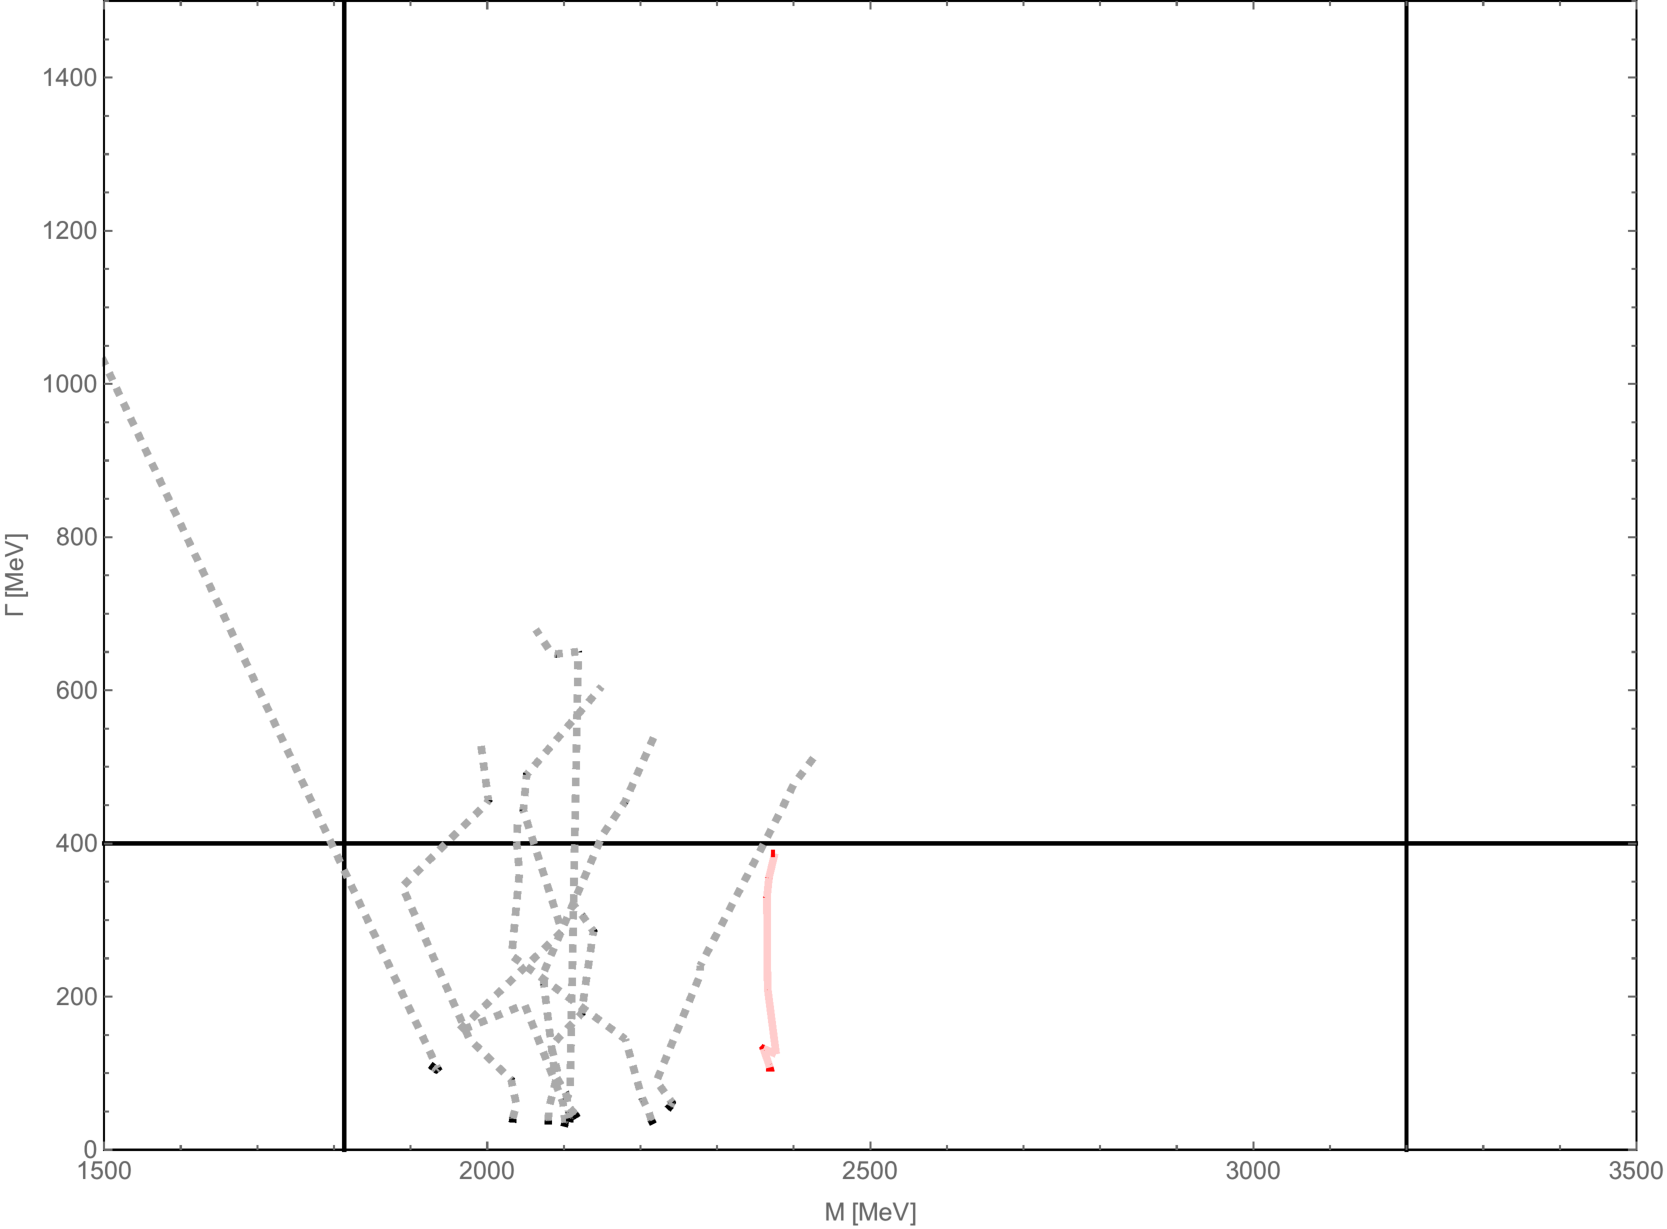
\includegraphics[width=0.99\linewidth]{Fig8B.pdf}
\caption{Resonance mass and width $\Gamma$ from fit to toy model. Resonances in red are the real ones and resonances in gray are superfluous. The resonances fade in brightness as the tuning parameter $\lambda$ increases. The vertical lines signify the mass cut off window while the horizontal line signifies the width cut off at 400 MeV.}
\label{fig:Fig8}
\end{center}
\end{figure}

\appendix
Considered (synthetic) data addresses the transition $\bar K^-p\to K\Xi$ via polarized and unpolarized differential cross sections 
(1 MeV$^2=389.4\,\text{b}$) given by
\begin{align}
\frac{d\sigma}{d\Omega}=(|g|^2+|h|^2) \frac{k_f}{k_i}
\qquad\text{ and }\qquad
\frac{d\sigma}{d\Omega}P=\frac{2 \space \text{Re}(g)h^{*}}{|g|^2+|h|^2} \, \frac{d\sigma}{d\Omega}\,,
\end{align}
where the moduli of the initial and final center of mass momenta are given by 
\begin{eqnarray}
&k_i=\frac{1}{2W}\sqrt{(W^2-(m_K-m_p)^2)(W^2-(m_K+m_p)^2)}\,,\\
&k_f=\frac{1}{2W}\sqrt{(W^2-(m_K-m_{\Xi})^2)(W^2-(m_K+m_{\Xi})^2)}\,,
\end{eqnarray}
respectively, for $W$ being the total energy of system, and $m$ denote the masses of the mesons and baryons. The latter are fixed to
\begin{align*}
m_{K}&=\frac{m_{K^{0}}+m_{K^{-}}+m_{K^{+}}}{3}
&\text{~~for~~}
&m_{K^{\pm}}=493.677 \text{ MeV}\,,
&m_{K^{0}}=497.648 \text{ MeV}\,,
\\
m_{\Xi}&=\frac{m_{\Xi^{0}}+m_{\Xi^{-}}}{2}
&\text{~~for~~}
&m_{\Xi^{-}}=1321.71 \text{ MeV}\,,
&m_{\Xi^{0}}=1314.86 \text{ MeV}\,,\\
&&~
&&m_p=938.27 \text{ MeV}\,.
%m_N=939.565 \text{ MeV}\,.
\end{align*}
The spin-flip and non-flip amplitudes $g_I$ and $h_I$ for the total Isospin of the reaction\footnote{$\braket{\Xi^0 K^0 | p K^-}= - \frac{1}{2}\braket{K\Xi(1,0)|\bar KN (1,0)}- \frac{1}{2}\braket{K\Xi(0,0)|\bar KN (0,0)}$ and 
{$\braket{\Xi^- K^+ | p K^-}= - \frac{1}{2}\braket{K\Xi(1,0)|\bar KN (1,0)}+ \frac{1}{2}\braket{K\Xi(0,0)|\bar KN (0,0)}$}} $I=0,1$ are related to the partial waves via

\begin{widetext}

\begin{align}
g_I&=\sum_{J=1}^{\text{jmax}} \frac{(2J+1)}{2 \sqrt{k_f  k_i}} \left[d^J_{\frac{1}{2} \frac{1}{2}}(\theta)[\tau^{J(J-\frac{1}{2})}_I+\tau^{J(J+\frac{1}{2})}_I]\cos(\frac{\theta}{2})+ d^J_{\frac{-1}{2} \frac{1}{2}}(\theta)[\tau^{J(J-\frac{1}{2})}_I-\tau^{J(J+\frac{1}{2})}_I]\sin(\frac{\theta}{2})\right]\,,\\
h_I&=-i\sum_{J=1}^{\text{jmax}} \frac{(2J+1)}{2 \sqrt{k_f  k_i}} \left[d^J_{\frac{1}{2} \frac{1}{2}}(\theta)[\tau^{J(J-\frac{1}{2})}_I+\tau^{J(J+\frac{1}{2})}_I]\sin(\frac{\theta}{2})- d^J_{\frac{-1}{2} \frac{1}{2}}(\theta)[\tau^{J(J-\frac{1}{2})}_I-\tau^{J(J+\frac{1}{2})}_I]\cos(\frac{\theta}{2})\right]\,.
\end{align}


For a given quantum numbers $(I,J,L)$, we assume the following general parametrization of the latter
\begin{align}
\tau(W)= \left(a\,e^{-\alpha^2 (\frac{k_f(W)}{\Lambda})^2} -x\,e^{i\Phi} \frac{\Gamma}{2(W-M+i \frac{\Gamma}{2})} \right) \left(\frac{k_f(W)}{\Lambda} \right) ^{L+\frac{1}{2}} \left( e^{i \phi} \right)\,,
\end{align}
where cutoff is fixed as $\Lambda=10^3 \text{ MeV}$, and $a,\alpha, \phi,\Phi,x, \Gamma,M$ are the free (real) parameters of the toy-model. Note that 
the latter are all different for different partial waves with the last four parameters describing resonance parameters.  


To avoid that the fit can perfectly reproduce the true solution, the synthetic data were generated using a slightly different parametrization (including an additional constant term $b$) of the background in the partial wave solutions,
\begin{align}
\tau(W)= \left((a+b\frac{k_f(W)}{\Lambda})\,e^{-\alpha^2 (\frac{k_f(W)}{\Lambda})^2} -x\,e^{i\Phi} \frac{\Gamma}{2(W-M+i \frac{\Gamma}{2})} \right) \left(\frac{k_f(W)}{\Lambda} \right) ^{L+\frac{1}{2}} \left( e^{i \phi} \right)\,.
\end{align}
These solutions were used at uniformly distributed $W$, and applying a perturbation with uniform Gauss error bars to generate the data. Furthermore, 4 resonances were included, appearing in the channels $S_{0,\frac{1}{2}}$, $P_{1,\frac{1}{2}}$, $D_{0,\frac{5}{2}}$, $D_{1,\frac{5}{2}}$. The partial waves corresponding to the data generated can be seen in  Fig.~\ref{fig:Fig1}, whereas the data itself can be seen in Figs.~\ref{fig:Fig2} and ~\ref{fig:Fig2x}.

\end{widetext}


%%%%%%%%%%%%%%%%%%%%%%%%%%%%%%%%%%%%%%%%%%%%%%%%%%%

\bibliography{stat}


\end{document}
